\documentclass[english]{../thermomemo/thermomemo}

\usepackage{amsmath, amsthm, amssymb}
\usepackage[T1]{fontenc}
\usepackage{graphicx}
\usepackage{mathtools}
\usepackage[utf8]{inputenc}
\usepackage{pgf}
\usepackage{tikz}
\usepackage{url}
\usepackage{enumerate}
\usepackage[font=small,labelfont=bf]{caption}
% For appendices
\usepackage[toc,page]{appendix}
\usepackage{xcolor}
\hypersetup{
  colorlinks,
  linkcolor={red!50!black},
  citecolor={blue!50!black},
  urlcolor={blue!80!black}
}

\title{Implementing MBWR and SPUNG equations of state in ThermoPack}
\author{Ailo Aasen}

% Package options
\usetikzlibrary{arrows,automata,decorations.markings,positioning}

\newcommand{\map}[3]{ #1 : #2 \to #3 }
\newcommand{\ip}[2]{\left\langle #1,\, #2 \right\rangle }
\newcommand{\norm}[1]{ \left\|{ #1 }\right\| }
\newcommand{\R}[0]{ \mathbb{R} }
\newcommand{\Q}[0]{ \mathbb{Q} }
\newcommand{\Z}[0]{ \mathbb{Z} }
\newcommand{\N}[0]{ \mathbb{N} }
\newcommand{\C}[0]{ \mathbb{C} }
\newcommand{\unitcircle}[0]{ \mathbb{S} }
\newcommand{\T}[0]{ \mathbb{T} }
\newcommand{\dd}[2]{\frac{\partial #1}{\partial #2}}
\newcommand{\mbn}[0]{\mathbf n}

\newcommand*{\pd}[2]{\frac{\partial #1}{\partial #2}}
\newcommand*{\pdd}[2]{\frac{\partial^2 #1}{\partial #2^2}}
\newcommand*{\pder}[2]{\left(\frac{\partial #1}{\partial #2}\right)}
\newcommand*{\pdder}[2]{\left(\frac{\partial^2 #1}{\partial #2^2}\right)}
\newcommand*{\pdersub}[3]{\left(\frac{\partial #1}{\partial #2}\right)_{#3}}
\newcommand*{\pddersub}[3]{\left(\frac{\partial^2 #1}{\partial #2^2}\right)_{#3}}
\newcommand*{\pdcross}[3]{\left(\frac{\partial^2 #1}{\partial #2 \partial #3}\right)}
\newcommand*{\pdcrosssub}[4]{\left(\frac{\partial^2 #1}{\partial #2 \partial #3}\right)_{#4}}

\newcommand*{\hF}[0]{\hat F}
\newcommand*{\hH}[0]{\hat H}

\newcommand{\mc}[1]{\mathcal{#1}}
\newcommand{\mcE}{ \mathcal{E}}
\newcommand{\mcF}{ \mathcal{F}}
\newcommand{\mcO}{ \mathcal{O}}
\newcommand{\mcU}{ \mathcal{U}}
\newcommand{\mcT}{ \mathcal{T}}
\newcommand{\mcL}{ \mathcal{L}}
\newcommand{\mcS}{ \mathcal{S}}

\newcommand{\paran}[1]{\left( #1 \right)}
\newcommand{\lp}{\left(}
  \newcommand{\rp}{\right)}

\newcommand{\dive}{\nabla \cdot}
\newcommand{\curl}{\nabla \times}

\newcommand{\sgn}{\operatorname{sgn}}
\newcommand{\sech}{\operatorname{sech}}
\newcommand{\cn}{\operatorname{cn}}
\newcommand{\clos}{\operatorname{clos}}
\newcommand{\id}{\operatorname{id}}
\newcommand{\ran}{\operatorname{ran}}
% \newcommand{\dim}{\operatorname{dim}}
\newcommand{\codim}{\operatorname{codim}}


% Number results section-wise
\newtheorem{thm}{Theorem}[section]
\newtheorem{defn}[thm]{Definition}
\newtheorem{cor}[thm]{Corollary}
\newtheorem{lem}[thm]{Lemma}
\newtheorem{prop}[thm]{Proposition}

% Number equations section-wise
\numberwithin{equation}{section}

% Misc
\newtheorem{definition}{Definition}
\newtheorem{theorem}{Theorem}
\newtheorem{case}{Case}
\tikzset{->-/.style={decoration={markings,mark=at position #1 with {\arrow{>}}},postaction={decorate}}}

\begin{document}
\frontmatter
\tableofcontents

\section{Introduction}
This memo documents the theory behind and ThermoPack-implementation of
the MBWR-19 and the MBWR-32 equations of state for pure fluids, as
well as their extension to mixtures via the SPUNG equation of
state. ThermoPack is a SINTEF Energy Research in-house thermodynamic library, and is
documented in Skaugen et al. \cite{ThermoPackDoc13}.

MBWR-19 and MBWR-32 are single-component equations of
state, having respectively $19$ and $32$ parameters fitted
to a specific substance. They are both examples of so-called
\textit{multiparameter equations of state}, and generally outperform
cubic equations of state when it comes to accuracy, but lose to them
in speed. MBWR-19 was first used by Bender (1970), and is also
referred to as the Bender equation. MBWR-32 is due to Jacobsen and
Stewart (1973), and is sometimes called the Jacobsen-Stewart equation,
or simply \textit{the MBWR equation}. The MBWR-19 and MBWR-32 have
been fitted to a range of components.

MBWR equations are often used as reference equations for so-called
\textit{Corresponding States} equations. The prevously implemented
Lee-Kesler equation of state, documented in Aarnes \cite{Aarnes13}, is
one example. Another Corresponding States equation is the SPUNG
equation. SPUNG stands for \textit{State Research and Development
  Program for Utilization of Natural Gas}, after the Norwegian state
program which partly financed the equation's development, and is
documented in J{\o}rstad \cite{Jorstad93}.

\subsection{How to implement equations of state in ThermoPack}
ThermoPack is a thermodynamics library which is documented in Skaugen et al.
\cite{ThermoPackDoc13}. The library has the convention of using $(T, P, \mbn)$ as
independent variables. For an equation of state to be considered implemented
in ThermoPack, the following is required: For each of the thermodynamic functions
\begin{itemize}
\item the compressibility $z$
\item the residual entropy $S^R$
\item the residual enthalpy $H^R$
\item the logarithmic fugacity coefficients $\ln \phi_i$
\end{itemize}
there should be routines which takes in temperature $T$, pressure $P$,
composition $\mbn$ and phase as input, and returns the values of these functions, as
well as the values of their first order partial derivatives when the independent
variables are $(T, P, \mbn)$.

In addition, a routine for calculating the residual Gibbs energy $G^r$
and its partial derivatives is usually desired.

When it comes to units, ThermoPack mostly uses base SI-units, e.g K
for temperature and Pa for pressure. An important exception is
molar volume and density, which are measured in
$\mathrm{dm}^3/\mathrm{mol}$ and $\mathrm{mol}/\mathrm{dm}^3$.



\section{Expressing thermodynamic functions using the reduced Helmholtz energy}

\subsection{Residual properties}
An arbitrary temperature-volume-composition state $(T,V,\mbn)$ can be reached by mixing
the pure fluids at temperature $T_0$ and approximately zero density and
pressure, heating the mixture to the temperature $T$ and then
compressing it to the volume $V$. It follows that the calculation of
an arbitrary thermodynamic property $M(T,V,\mbn)$ can be split up
according to
\begin{equation}
  \label{M_TVN}
  M = (\Delta M^\star)_{\text{mixing}} + \int_{T_0}^T \lp
  \frac{\partial M^\star}{\partial T} \rp_{V=\infty,\mbn} dT +
  \int_{\infty}^V \lp \frac{\partial M}{\partial V} \rp_{T,\mbn} dV
\end{equation}
where $M^\star$ denotes the property at zero density and pressure, and $(\Delta M^\star)_{\text{mixing}}$ denotes the property due to
mixing at zero density and pressure.

If instead $(T,P,\mbn)$ are used as independent variables, the
equivalent of \eqref{M_TVN} is
\begin{equation}
  \label{M_TPN}
  M = \Delta M^\star + \int_{T_0}^T \lp \frac{\partial M^\star}{\partial
    T} \rp_{P=0,\mbn} dT + \int_{0}^P \lp \frac{\partial M}{\partial P}
  \rp_{T,\mbn} dP.
\end{equation}
The right-hand sides of \eqref{M_TVN} and \eqref{M_TPN} can be
rearranged to comprise two terms, one which is the property $M^\star$
of the hypothetical perfect gas at the state $(T,V,\mbn)$ or
$(T,P,\mbn)$ over some fixed, chosen zero, and a second term $M^R = M
- M^\star$, called the residual. From its definition $M^R = M -
M^\star$, we see that the residual $M^R$ must be defined as
\begin{equation}
  \label{eq:ResDef}
  \begin{aligned}
    M^R(T,V,\mbn) &= \int_\infty^V \left[ \lp \dd{M}{V_1} \rp_{T,\mbn} -
      \lp \dd{M^\star}{V_1} \rp_{T,\mbn} \right] dV_1, \\
    M^R(T,P,\mbn) &= \int_0^P \left[ \lp \dd{M}{P_1} \rp_{T,\mbn} - \lp
      \dd{M^\star}{P_1} \rp_{T,\mbn} \right] dP_1.
  \end{aligned}
\end{equation}
Beware that in general we have $M^R(T,V,\mbn) \neq
M^R(T,P,\mbn)$. This may seem strange since the value of a
thermodynamic property shouldn't depend on which coordinates one
happens to use; for example it is of course always true that
$M(T,P,\mbn) = M(T,V,\mbn)$. The reason this equality does not hold
for residual properties is that having temperature, volume and
composition $(T,V,\mbn)$ as a perfect gas state, is not the same the
same perfect gas state as having temperature, pressure and composition
$(T,P,\mbn)$, because in general $PV \neq nRT$, and thus $M^\star(T,V,\mbn) \neq
M^\star(T,P,\mbn)$

\subsection{Relating thermodynamic functions functions to $F$}
Let
$$
A = -PV + \sum \mu_i n_i
$$
denote the Helmholtz energy of an arbitrary fluid. We have $dA =
-SdT-PdV + \sum_i \mu_i dn_i$, and the natural variables for $A$ are
$T, V, \mbn$, all of which are accessible variables (in contrast to
e.g. entropy). Let as above $A^R$ denote the residual Helmholtz
energy. Then from \eqref{eq:ResDef} we see that
\begin{equation}
  \label{eq:1}
  A^R(T,V,\mbn) = \int_\infty^V \lp -P(T,V_1,\mbn) + nRT/V_1 \rp dV_1.
\end{equation}

A quantity of prime importance is the \textit{reduced} residual
Helmholtz energy, defined as
\begin{equation}
  \label{eq:Fdef}
  F(T,V,\mbn) = \frac{A^R(T,V,\mbn)}{RT}
\end{equation}
In modern thermodynamic engineering, equations of state are usually
formulated as an expression for $F$ as a function of temperature and
volume. Note that $F$ is written as a function of $(T,V,\mbn)$, and
indeed explicit functional expressions for $F$ are usually only
obtainable in these variables. Thus if one wants to compute $F$ from
knowledge only of $(T,P,\mbn)$, one first has to compute $V$. For all
but the simplest equations of state (like e.g. cubic equations), this has
to be done using an iterative solver, and can be a time-consuming part
of the program. See also section \ref{sec:density}.

When we are dealing with pure fluids, which after all is the setting
of the MBWR equations, we have $\mbn = n$, where $n$ is the total
number of moles of the pure fluid, and it is more convenient to
consider extensive properties such as $F$ on a per mole (molar)
basis. In this setting it is natural to use density $\rho = n/V$ as a
variable (or alternatively, molar volume $v = 1/\rho$). Indeed, the MBWR
equations are usually formulated as equations for the pressure $P =
P(T,\rho)$. They are easily converted -- using \eqref{eq:Fdef} -- to
an equation for the molar Helmholtz energy $\alpha$ as a function of
$(T,\rho)$, where $\alpha$ is defined as:
\begin{align}
  \alpha(T,\rho) &= \frac{A^R(T,n/\rho,n)}{nRT} \\
  &= \frac{F(T,n/\rho,n)}{n},
\end{align}
where the functions on the right hand sides are the ones in equation
\eqref{eq:Fdef}. Note that $F$ has units $\mathrm{mol}$, while
$\alpha$ is adimensional.
% Seeing as the right side expressions in is independent of $n$, one
% usually thinks of $n$ as being $1$.

If one has an equation for $F$, it turns out that all thermodynamic
properties can be computed from $F$ and its partial
derivatives. Below, the thermodynamic functions needed in ThermoPack, together with their first
order partials, are given in terms of $F$ and its first and second
order partial derivatives.

\subsubsection*{Compressibility factor}
\noindent
The compressibility factor $z$ is a dimensionless number which can be
written in several equivalent forms:
\begin{equation}
  \label{eq:zDef}
  z = \frac{PV}{nRT} = \frac{Pv}{RT} = \frac{P}{\rho RT}  = \frac{v}{v_{ig}}
\end{equation}
In the equation \eqref{eq:zDef} $v = V /n$ is the specific molar
volume, $\rho = 1/v$ is the molar density, $v_{ig}$ is the specific
volume of an ideal gas, $R$ is the universal gas constant, and $P$,
$V$, $T$ and $n$ are pressure, volume, temperature and total number of
moles of the fluid, respectively. For ideal gases $z=1$ for all $T$
and $P$ and $n$, wheras for real gases $z$ is a non-constant function
of $T$ and $P$ and $n$.

\subsubsection*{Residual entropy}
\begin{equation}
  \label{eq:Sres}
  S^R(T,P,n) = nR \ln z - RF - RT \lp \dd{F}{T} \rp_{V,n}. % Double-checked
\end{equation}

\subsubsection*{Residual enthalpy}
\begin{equation}
  \label{eq:Hreduced}
  H^R(T,P,n) = -RT^2 \lp \dd{F}{T} \rp_{V,n} + PV - nRT, % Double-checked
\end{equation}

\subsubsection*{Logarithmic fugacity coefficent}
\begin{equation}
  \label{eq:lnphireduced}
  \ln \phi_i(T,P,n) = \lp \dd{F}{n_i} \rp_{T,V} - \ln z. % Double-checked
\end{equation}

\subsection{Partial derivatives of the thermodynamic properties}
The following formulas are mostly taken directly from Aarnes
\cite{Aarnes13}.
\subsubsection*{Pressure}
To simplify the notation in the following derivatives, a relation
between the pressure and its derivatives, and the reduced residual
Helmholtz function is introduced.

\begin{equation}
  \label{def:P}
  P(T,V,\textbf{n}) = -RT \left( \frac{\partial F}{\partial V} \right)_{T, \textbf{n}} + \frac{nRT}{V}
\end{equation}

The partial derivatives of the pressure, with respect to temperature,
volume and composition, respectively, are given by:
\begin{align}
  \label{eq:P_T}
  & \pder{P}{T}_{V, \textbf{n}} = \frac{P}{T} - RT \pdcross{F}{T}{V}_{n_i} \\
  \label{eq:P_V}
  & \pder{P}{V}_{T, \textbf{n}} = -RT \pdder{F}{V}_{T, \textbf{n}} - \frac{nRT}{V^2} \\
  \label{eq:P_i}
  & \pder{P}{n_i}_{T,V} = -RT \pdcross{F}{n_i}{V}_T + \frac{RT}{V}
\end{align}

Furthermore, the partial derivatives of the volume with respect to
composition and temperature are defined, by the use of the triple
product rule and the derivatives of the pressure:
\begin{align}
  \label{def:V_i}
  \bar{V}_i \equiv \pder{V}{n_i}_{T,P} =  - \frac{\pder{P}{n_i}_{T,V}}{\pder{P}{V}_{T,\textbf{n}}} \\
  \label{def:V_T}
  \bar{V}_T \equiv \pder{V}{T}_{P,\textbf{n}} = -
  \frac{\pder{P}{T}_{V,\textbf{n}}}{\pder{P}{V}_{T,\textbf{n}}}
\end{align}

The following derivatives are all carried out for functions that are
$(T,P,\textbf{n})$-states, that is $z = z(T,P,\textbf{n})$, $S^R =
S^R(T,P,\textbf{n})$, $H^R = H^R(T,P,\textbf{n})$ and $\ln \phi_i =
\ln \phi_i(T,P,\textbf{n})$. Several of these calculations get rather
involved, and only the resulting expressions are presented here.

\subsubsection*{Compressibility}
\begin{align}
  \label{eq:z_T}
  & \left( \frac{\partial z}{\partial T} \right)_{P, \textbf{n}} = -z\left[\frac{1}{T} - \frac{\bar{V}_T}{V}\right] \\
  \label{eq:z_P}
  & \left( \frac{\partial z}{\partial P} \right)_{T, \textbf{n}} = z \left[ \frac{1}{P} + \frac{1}{V \pder{P}{V}_{T,\textbf{n}}} \right] \\
  \label{eq:z_i}
  & \left( \frac{\partial z}{\partial n_i} \right)_{T,P} = - z \left[
    \frac{1}{n} - \frac{\bar{V}_i}{V} \right]
\end{align}

\subsubsection*{Entropy}
\begin{align}
  \label{eq:S^R_T}
  & \pder{S^R(T,P,\textbf{n})}{T}_{P,\textbf{n}} = \bar{V}_T \pder{P}{T}_{V,\textbf{n}} - R \left[2\pder{F}{T}_{V,\textbf{n}} + T \pdder{F}{T}_{V,\textbf{n}} + \frac{n}{T} \right] \\
  \label{eq:S^R_P}
  & \pder{S^R(T,P,\textbf{n})}{P}_{T,\textbf{n}} = \frac{nR}{P} - \bar{V}_T \\
  \label{eq:S^R_i}
  & \pder{S^R(T,P,\textbf{n})}{n_i}_{T,P} = \bar{V}_i
  \pder{P}{T}_{V,\textbf{n}} - R\left[ \pder{F}{n_i}_{T,V} +
    T\pdcross{F}{T}{n_i}_V + 1 - \ln z \right]
\end{align}

\subsubsection*{Enthalpy}
\begin{align}
  \label{eq:H^R_T}
  & \pder{H^R}{T}_{P, \textbf{n}} = \bar{V}_T T \pder{P}{T}_{V,\textbf{n}} - RT \left[ 2\pder{F}{T}_{V,\textbf{n}} + T \pdder{F}{T}_{V,\textbf{n}} + \frac{n}{T} \right] \\
  \label{eq:H^R_P}
  & \pder{H^R}{P}_{T, \textbf{n}} = V - T \bar{V}_T \\
  \label{eq:H^R_i}
  & \pder{H^R}{n_i}_{T,P} = \bar{V}_i T \pder{P}{T}_{V,\textbf{n}}
  -RT^2 \pdcross{F}{T}{n_i}_V - RT
\end{align}

\subsubsection*{Fugacity coefficients}
\begin{align}
  \label{eq:lnphi_T}
  & \pder{\ln \phi_i}{T}_{P, \textbf{n}} = \pdcross{F}{T}{n_i}_V + \frac{1}{T} - \frac{\bar{V}_i}{RT}  \pder{P}{T}_{V,\textbf{n}} \\
  \label{eq:lnphi_P}
  & \pder{\ln \phi_i}{P}_{T, \textbf{n}} = \frac{\bar{V}_i}{RT} - \frac{1}{P} \\
  \label{eq:lnphi_i}
  & \pder{\ln \phi_i}{n_j}_{T, P} = \pdcross{F}{n_j}{n_i}_{T,V} +
  \frac{1}{n} + \frac{\pder{P}{V}_{T,\textbf{n}}}{RT} \bar{V}_j
  \bar{V}_i
\end{align}

\subsubsection*{Gibbs energy}
Residual Gibbs energy is not documented in Aarnes \cite{Aarnes13} and
is therefore documented here. From Michelsen \cite{Michelsen07} we
have
$$
G^R(T,P,\mbn) = RT F(T,V,\mbn) + PV - nRT(1 + \ln z),
$$
whence
\begin{align}
  % \label{eq:}
  % & \pder{G^R}{T}_{P, \textbf{n}} = R \lp F + T
  % \pdersub{F}{T}{V,\mbn} + T \pdersub{F}{V}{T,\mbn} \bar{V}_T
  % -n(1+\ln z) \rp + \lp P - \frac{nRT}{V} \rp \bar{V}_T \\
  % & \pder{G^R}{T}_{P, \textbf{n}} = R \lp F + T
  % \pdersub{F}{T}{V,\mbn} + T \pdersub{F}{V}{T,\mbn} \bar{V}_T + P
  % \rp \\
  & \pder{G^R}{T}_{P, \textbf{n}} = R \lp F + T \pdersub{F}{T}{V,\mbn} - n \ln z \rp + \lp P - P/z + RT \pdersub{F}{V}{T,\mbn} \rp \bar{V}_T \\
  % & \pder{G^R}{P}_{T, \textbf{n}} = RT \pdersub{F}{V}{T,\mbn} \bar
  % V_P + P \bar V_P + V - nRT \lp \frac{1}{P} + \frac{\bar V_P}{V}
  % \rp \\
  & \pder{G^R}{P}_{T, \textbf{n}} = V - \frac{nRT}{P} \\
  % & \pder{G^R}{n_i}_{T, P} = RT \pdersub{F}{V}{T,\mbn} \bar V_i + P
  % \bar V_i + RT \pdersub{F}{n_i}{T,P} - RT (1+\ln z) + RT -
  % \frac{nRT}{V} \bar V_i
  & \pder{G^R}{n_i}_{T, P} = RT \lp \pdersub{F}{n_i}{T,P} - \ln z \rp
\end{align}

\subsubsection*{Internal energy}
Residual internal energy is not documented in Aarnes \cite{Aarnes13} and
is therefore documented here. We have
$$
U^R(T,P,\mbn) = nRT \ln z - RT^2 \lp \dd{F}{T} \rp_{V,n}
$$
and thus
\begin{align}
  & \pder{U^R}{T}_{P, \textbf{n}} = nR \left[ \ln z + \frac{T \bar
      V_T}{V} -1 \right] - RT\lp 2 \pder{F}{T}_{V,\mbn} + T\pdder{F}{T}_{V,\mbn} \rp \\
  & \pder{U^R}{P}_{T, \textbf{n}} = nTR\left[ \frac{1}{P} + \frac{1}{V
      \pder{P}{V}_{T,\mbn}} \right] - \frac{RT^2\pdcross{F}{T}{V}_\mbn}{\pder{P}{V}_{T,\mbn}}\\
  & \pder{U^R}{n_i}_{T, P} = TR \left[ \ln z + \frac{n\bar V_i}{V}
    -1\right] - RT^2 \pdcross{F}{T}{n_i}_V
\end{align}

\subsection{Relating $F$-derivatives to $\alpha$-derivatives}
In the case of pure fluids, it is as mentioned more convenient to use
the function $\alpha$ defined by
\begin{equation}
  F(T,V,n) = n \alpha(T, \rho).
\end{equation}
This implies the following relations between the derivatives of $F$
and the derivatives of $\alpha$.

\subsubsection*{$T$-derivatives}
\begin{align}
  \label{eq:DFDT}
  & \pder{F}{T}_{V, n} = n \pder{\alpha}{T} \\
  \label{eq:D2FDT2}
  & \pdder{F}{T}_{V, n} = n \pdder{\alpha}{T}
\end{align}

\subsubsection*{$V$-derivatives}
\begin{align}
  \label{eq:DFDV}
  & \pder{F}{V}_{T, n} = -\frac{n^2}{V^2} \pder{\alpha}{\rho} \\
  \label{eq:D2FDV2}
  & \pdder{F}{V}_{T, n} = \frac{2n^2}{V^3} \pder{\alpha}{\rho} +
  \frac{n^3}{V^4} \pdder{\alpha}{\rho}
\end{align}

\subsubsection*{$n$-derivatives}
\begin{align}
  \label{eq:DFDn}
  & \pder{F}{n}_{V, n} = \alpha + \frac{n}{V}\pder{\alpha}{\rho} \\
  \label{eq:D2FDn2}
  & \pdder{F}{n}_{V, n} = \frac{2}{V} \pder{\alpha}{\rho} +
  \frac{n}{V^2} \pdder{\alpha}{\rho}
\end{align}

\subsubsection*{Cross-derivatives}
\begin{align}
  \label{eq:D2FDTV}
  & \pdcross{F}{T}{V}_{V} = -\frac{n^2}{V^2} \pdcross{\alpha}{T}{\rho} \\
  \label{eq:D2FDTn}
  & \pdcross{F}{T}{n}_{V, n} = \pder{\alpha}{T} + \frac{n}{V} \pdcross{\alpha}{T}{\rho} \\
  \label{eq:D2FDVn}
  & \pdcross{F}{V}{n}_{V, n} = -\frac{2n}{V^2} \pder{\alpha}{\rho} -
  \frac{n^2}{V^3} \pdder{\alpha}{\rho}
\end{align}

\section{The MBWR equations of state}
Both the MBWR-19 and the MBWR-32 equations of state take the general
form
\begin{equation}
  \label{eq:MBWRform}
  P(T,\rho) = \rho R T + \sum_{k=1}^{I_{\mathrm{pol}}} a_k T^{t_k} \rho^{d_k} +\sum_{k=I_{\mathrm{pol}}+1}^{I_{\mathrm{tot}}} a_k T^{t_k} \rho^{d_k} \exp \lp -\gamma \rho^2 \rp.
\end{equation}
The last sum on the right hand side of \eqref{eq:MBWRform} side is referred
to as the exponential part, and the rest is called the polynomial
part%
\footnote{This is somewhat misleading, since not all the $t_k$ are
  positive integers.}. %
The $d_k$ are positive integers and the $t_k$ are rational numbers,
both inherent to the equation of state. Their values are given in
Table 1 for MBWR-19, and in Table 2
for MBWR-32. The parameters $a_1,\ldots,a_{I_{\mathrm{tot}}}$ are not
inherent to the equation of state, but are substance-specific and thus have to be fitted to experimental measurements. For MBWR-19 and MBWR-32 we have
$I_{\mathrm{tot}}$ equal to $19$ and $32$, respectively. The
parameter $\gamma$ usually equals $1/\rho_{c}^2$, but may have been
fitted with something else. In any case, even though $\gamma$ is
component dependent, it is not optimized in the fitting process, which
is the reason it is not counted as a bona fide parameter. MBWR-19 is
however only \textit{our} choice of name, and other sources (e.g.
J{\o}rstad \cite{Jorstad93}) instead calls it MBWR-$20$.

Note that, for both MBWR-19 and MBWR-32, all the density exponents $d_k$ are positive. This is not coincidental, but a necessity to make it have the desired asymptotic behavior
$$
\lim_{\rho \to 0} P(T,\rho) = 0.
$$

The MBWR equations are sometimes written with terms grouped according
to powers of $\rho$:
\begin{equation}
  \label{eq:bpbeform}
  P(T,\rho) = \sum_{i=1}^{BP_\text{len}}BP_i(T) \cdot \rho^i
  + \exp(-\gamma \rho^2) \sum_{i=1}^{BE_\text{len}} BE_i(T) \cdot \rho^{2i+1}.
\end{equation}
This aggregation of the temperature dependents terms is sometimes
convenient, because one often wants to evaluate $P(T,\rho)$ for the same $T$
but several different $\rho$, the prime example being the iterative procedure in the density
solver, see section \ref{sec:density}. In this case it is
computationally efficient to pre-calculate the coefficients $BP_i(T)$
and $BE_i(T)$.

\begin{table}
  \label{BenderTerms}
  \centering
  \begin{tabular}{c c c c | c c c c }
    $k$		& $d_k$		& $t_k$		& type		 & k		& $d_k$		& $t_k$		& type		   \\
    \hline
    $1$		& $2$       	&$ 1$		& pol              & $11$		& $5$       	&$ 1$		&pol                 \\
    $2$		& $2$       	&$ 0$		&pol               & $12$		& $5$       	&$ 0$		&pol                  \\
    $3$		& $2$       	&$-1$		&pol               & $13$		& $6$       	&$ 0$		&pol                  \\
    $4$		& $2$       	&$-2$ 		&pol               & $14$		& $3$       	&$ 0$		& exp              \\
    $5$		& $2$       	&$-3$ 		&pol               & $15$		& $3$       	&$-1$		& exp              \\
    $6$		& $3$       	&$ 1$		&pol               & $16$		& $3$       	&$-2$		& exp              \\
    $7$		& $3$       	&$ 0$		&pol               & $17$		& $5$       	&$ 0$		& exp              \\
    $8$		& $3$       	&$-1$		&pol               & $18$		& $5$       	&$-1$		& exp              \\
    $9$		& $4$       	&$ 1$		&pol               & $19$		& $5$       	&$-2$		& exp              \\  
    $10$	& $4$       	&$ 0$		&pol               &               &               &               &
  \end{tabular}
  \caption{Overview of inherent parameters in the MBWR-$19$ model. $I_{\mathrm{pol}}=13$, $I_{\mathrm{tot}}=32$.}
\end{table}

\begin{table}
  \label{MBWR32Terms}
  \centering
  \begin{tabular}{c c c c | c c c c }
    $k$		        & $d_k$		& $t_k$		& type		& k		 & $d_k$	  & $t_k$	    & type	       \\
    \hline
    $1$		        & $2$       	&$ 1$		& pol           & $17$	 & $8$       	  &$-1$		    & pol              \\
    $2$		        & $2$       	&$ 0.5$		&pol            & $18$	 & $8$       	  &$-2$		    & pol              \\
    $3$		        & $2$       	&$ 0$		&pol            & $19$	 & $9$       	  &$-2$		    & pol              \\
    $4$		        & $2$       	&$-1$ 		&pol            & $20$	 & $3$       	  &$-2$		    & exp              \\
    $5$		        & $2$       	&$-2$ 		&pol            & $21$	 & $3$       	  &$-3$		    & exp              \\
    $6$		        & $3$       	&$ 1$		&pol            & $22$	 & $5$       	  &$-2$		    & exp              \\
    $7$		        & $3$       	&$ 0$		&pol            & $23$	 & $5$       	  &$-4$		    & exp              \\
    $8$		        & $3$       	&$-1$		&pol            & $24$	 & $7$       	  &$-2$		    & exp              \\
    $9$		        & $3$       	&$-2$		&pol            & $25$	 & $7$       	  &$-3$		    & exp              \\
    $10$		& $4$       	&$ 1$		&pol            & $26$	 & $9$        	  &$-2$		    & exp              \\
    $11$		& $4$       	&$ 0$		&pol            & $27$   & $9$            &$-4$             & exp              \\
    $12$		& $4$       	&$-1$		&pol            & $28$   & $11$           &$-2$             & exp              \\
    $13$		& $5$       	&$ 0$		&pol            & $29$   & $11$           &$-3$             & exp              \\
    $14$		& $6$       	&$-1$		&pol            & $30$   & $13$           &$-2$             & exp              \\
    $15$		& $6$       	&$-2$		&pol            & $31$   & $13$           &$-3$             & exp              \\
    $16$		& $7$       	&$-1$		&pol            & $32$   & $13$           &$-4$             & exp              
  \end{tabular}
  \caption{Overview of inherent parameters in the MBWR-$32$ model. $I_{\mathrm{pol}}=19$, $I_{\mathrm{tot}}=32$.}
\end{table}

% \section{Implementation}
% The component dependent correlated parameters have been fetched from
% the tplib library, more precisely the text file
% \textit{corr.inp}. Instead of reading the parameters from a text
% file each time an MBWR model is initiated, all the parameters are
% stored in a compiled module. Since the number of component models
% was relatively small ($63$ models for MBWR-32 and MBWR-19 combined),
% the parameter data was copied manually into the code, where it
% initialises a Fortran TYPE holding the data.
% 
% It is wise to precalculate the temperature dependent coefficients
% early on, and don't calculate them again and again. This is done in
% MBWR_coef

\section{Database for the MBWR substance-specific parameters}
The correlated values of $a_k$ for various substances are stored in
the file \textit{tpmbwrdata.f90}, and have been retrieved from the old
TPlib thermodynamics library. In the current database $9$ substances
have correlations for MBWR-32, while $54$ substances have
correlations for MBWR-19.

It is important to understand exactly what these coefficients in the
database mean. Let us first consider the MBWR-32 equation. For
MBWR-32, each correlation in the database consists of 33 coefficients
$(a_1,\ldots,a_{32},\gamma)$, which fit into the equation as follows (see
J{\o}rstad \cite{Jorstad93}):
\begin{align*}
  P(T,\rho) = \sum_{i=1}^{19} BP_i \cdot \rho^i + e^{-\gamma \rho^2}
  \sum_{i=1}^{6} BE_i \cdot \rho^{2i+1}.
\end{align*}
where
\begin{equation}
  \label{eq:BPBE_MBWR32}
  \begin{aligned}
    BP_1 &= RT \\
    BP_2 &= a_1T+a_2T^{1/2}+a_3+a_4/T+a_5/T^2 \\
    BP_3 &= a_6T+a_7+a_8/T+a_9/T^2 \\
    BP_4 &= a_{10}T+a_{11}+a_{12}/T \\
    BP_5 &= a_{13} \\
    BP_6 &= a_{14}/T+a_{15}/T^2 \\
    BP_7 &= a_{16}/T \\
    BP_8 &= a_{17}/T+a_{18}/T^2 \\
    BP_9 &= a_{19}/T^2 \\
    BE_1 &= a_{20}/T^2+a_{21}/T^3 \\
    BE_2 &= a_{22}/T^2+a_{23}/T^4 \\
    BE_3 &= a_{24}/T^2+a_{25}/T^3 \\
    BE_4 &= a_{26}/T^2+a_{27}/T^4 \\
    BE_5 &= a_{28}/T^2+a_{29}/T^3 \\
    BE_6 &= a_{30}/T^2+a_{31}/T^3 + a_{32}/T^4.
  \end{aligned}
\end{equation}
Here $P$ is measured in Pascal, $T$ is
measured in Kelvin and $\rho$ is measured in moles per litre -- the
convention in ThermoPack.


Let us next consider the MBWR-19 equation. In the database each
substance has associated with it an array of $20$ parameters
$(a_1,\ldots,a_{19},\gamma)$ with the property that (see Polt \cite{Polt87})
\begin{align*}
  P(T,\rho) = BP_1 \rho + \left[ BP_2 \rho^2 + BP_3 \rho^3 + BP_4
    \rho^4 + BP_5 \rho^5 + BP_6 \rho^6 + (BE_1\rho^3 + BE_2 \rho^5)
    e^{-\gamma \rho^2} \right] \cdot 10^3,
\end{align*}
where
\begin{equation}
  \label{eq:BPBE_MBWR19}
  \begin{aligned}
    BP_1 &= RT \\
    BP_2 &= a_1T-a_2-a_3/T-a_4/T^2-a_5/T^3 \\
    BP_3 &= a_6T+a_7+a_8/T \\
    BP_4 &= a_9T+a_{10} \\
    BP_5 &= a_{11}T+a_{12} \\
    BP_6 &= a_{13} \\
    BE_1 &= a_{14}/T^2+a_{15}/T^3+a_{16}/T^4 \\
    BE_2 &= a_{17}/T^2+a_{18}/T^3+a_{19}/T^4.
  \end{aligned}
\end{equation}
Take note of the factor $10^3$, as well as the sign inversions for
terms $a_2,a_3,a_4,a_5$. Also for MBWR-19, $P$ is measured in Pascal, $T$ is
measured in Kelvin and $\rho$ is measured in moles per litre.

\subsubsection*{No MBWR data set for $CO_2$}
Although there was a data set for $\mathrm{CO}_2$ for MBWR-19 in the old TPlib
library, it is wrong. According to this data set, $\mathrm{CO_2}$ is still
subcritical at $310$ K, which is about $5$ K over its measured critical
temperature. VLE calculations using SPUNG with $\mathrm{CO}_2$ as reference
component also gives absurd results. Although the dissertation by Polt \cite{Polt87}
has been checked, he surprisingly doesn't give a correlation for
$\mathrm{CO}_2$. The correlation in the TPlib database has no reference.

\section{The MBWR density solver} \label{sec:density}
When the MBWR equations of state are called from ThermoPack, the
temperature, pressure and the phase is usually what
is given as input. However, the independent variables in MBWR
equations are density and temperature, not temperature and
pressure. Therefore, an algorithm which takes in $T$ and $P$ and
solves for $\rho$ is needed.

The density solver in the old thermodynamics library, TPlib, was not as robust as
desired. Jørstad writes the following in his thesis \cite{Jorstad93}:
\textit{Calculation of the density results sometimes in an incorrect
  solution or in a few circumstances breaks down (...) Approximately 1
  out of 500 calculations fails.} A better density solver is therefore
required. This section discusses the theory behind the implementation
of a new, more robust density solver.

In this section $T_0$ and $P_0$ will denote arbitrary but fixed
temperatures and pressures.

\subsection{Phases and the correct density root} % Bad title...
A typical plot of the function $\rho \mapsto P(T_0,\rho)$ is given in
Figure \ref{fig:p_ill}. As illustrated by this graph, there will
from a purely mathematical standpoint be several choices of $\rho$
which satisfies $P(\rho,T_0) = P_0$. However, not all of these
densities correspond to a physically realistic state. A first
criterion for the density being a physical solution is that belongs to
some interval over which $P(T_0,\rho)$ is positive and
increasing. This is due to the fact that, at a given temperature,
higher pressure will always correspond to a higher density. Applying
this first criterion, we see that there are two candidates for the
physically correct density. To choose the correct one of these two, we
need to know what phase, gas or liquid, the fluid is in: the gas phase
corresponds to the lowest density, the liquid phase corresponds to the
highest density. Let us call the part of the graph corresponding to
valid vapor densities the ``vapor hill'', and similarly call the part of the
graph corresponding to liquid solutions the ``liquid hill''. Thus,
given the phase, one has to choose the solution lying on the
corresponding hill.

\begin{figure}[h]
  \centering
  \includegraphics[width=0.7\textwidth]{figures/pressureIllustration.eps}
  \caption{A log-log plot of the MBWR-19 density-pressure curve for CH$_4$ and a
    subcritical temperature, and an example input pressure (green) drawn
    in. Where $P(T_0,\rho)$ becomes negative we have plotted
    $|P(T_0,\rho)$ in red.}
  \label{fig:p_ill}
\end{figure}

The choice of root is even easier for supercritical temperatures, $T_0
> T_c$, as illustrated in Figure \ref{fig:p_ill_sup}. In this
case there is only one interval where $P(T_0,\rho)$ is increasing, and
so the density is independent of phase. Physically, this reflects the
fact that for supercritical temperatures, there is no discontinuous
phase change.

\begin{figure}[h]
  \centering
  \includegraphics[width=0.7\textwidth]{figures/pressureIllustrationSupercritical.eps}
  \caption{The MBWR-19 density-pressure curve for CH$_4$ and a supercritical temperature, and
    an example input pressure drawn in.}
  \label{fig:p_ill_sup}
\end{figure}

A case where it is not so straightforward how choose the physical
density is shown in Figure \ref{fig:p_ill_meta}. If the user inputs liquid
phase, the question is whether one should return the solution
corresponding to the gas phase, or the density corresponding to the
liquid phase having minimum pressure.

\begin{figure}[h]
  \centering
  \includegraphics[width=0.7\textwidth]{figures/pressureIllustrationMeta.eps}
  \caption{The MBWR-19 density-pressure curve for CH$_4$ and a
    temperature below but close to the critical temperature, and an example input pressure drawn in.}
  \label{fig:p_ill_meta}
\end{figure}

Sometimes the user may not want to give the algorithm an input phase,
but rather ask that it chooses the phase which corresponds to the physically
stable solution. This is possible by letting the algorithm search for
both the liquid and gas root, and then returning the density
corresponding to minimum Gibb's energy.

\subsection{The density solver algorithm}
Although we tried many algorithms (e.g. the Illonois algorithm, the
Pegasus method, Halley's method), in the end the best method
proved to be Newton's method. A major reason for its speed is that
it is cheap to calculate the derivative $\partial_\rho P(T_0,\rho)$ by precalculating the temperature dependent coefficients, and
that if one evaluates both $P(T_0,\rho)$ and its derivative at the
same point, much of the computation overlaps, allowing a considerable
speedup compared to computing each of them separately. (Of course, the same overlap occurs when computing the second derivative.)

The never-ending worry with Newton's method is that it may shoot off
and not converge to the desired root. But there are special cases where
Newton's method is guaranteed to converge:
\begin{enumerate}
\item If a function is concave and increasing and the initial guess is
  smaller than the root, then Newton's method is guaranteed to
  converge, and the rate of convergence is quadratic.
\item If a function is convex and increasing and the initial guess is
  larger than the root, then Newton's method is guaranteed to
  converge, and the rate of convergence is quadratic.
\end{enumerate}

This of course requires us to know something about the convexity of $P(T_0,\rho)$. Interestingly, by plotting
$\partial^2P(T_0,\rho)/\partial\rho^2$ and $P(T_0,\rho)$ together, we have found evidence
for the ``gas hill'' being concave and increasing, and the ``liquid
hill'' being convex and increasing%
\footnote{A possible physical interpretation: When density is
  low, increasing pressure increases density little at first, but then
  more and more as long-range attraction becomes significant. When
  density is high, increasing pressure increases density less and less
  as short-term repulsion becomes dominant.}. %
An example is shown in Figure \ref{convexityPlot}.
\begin{figure}[h]
  \centering
  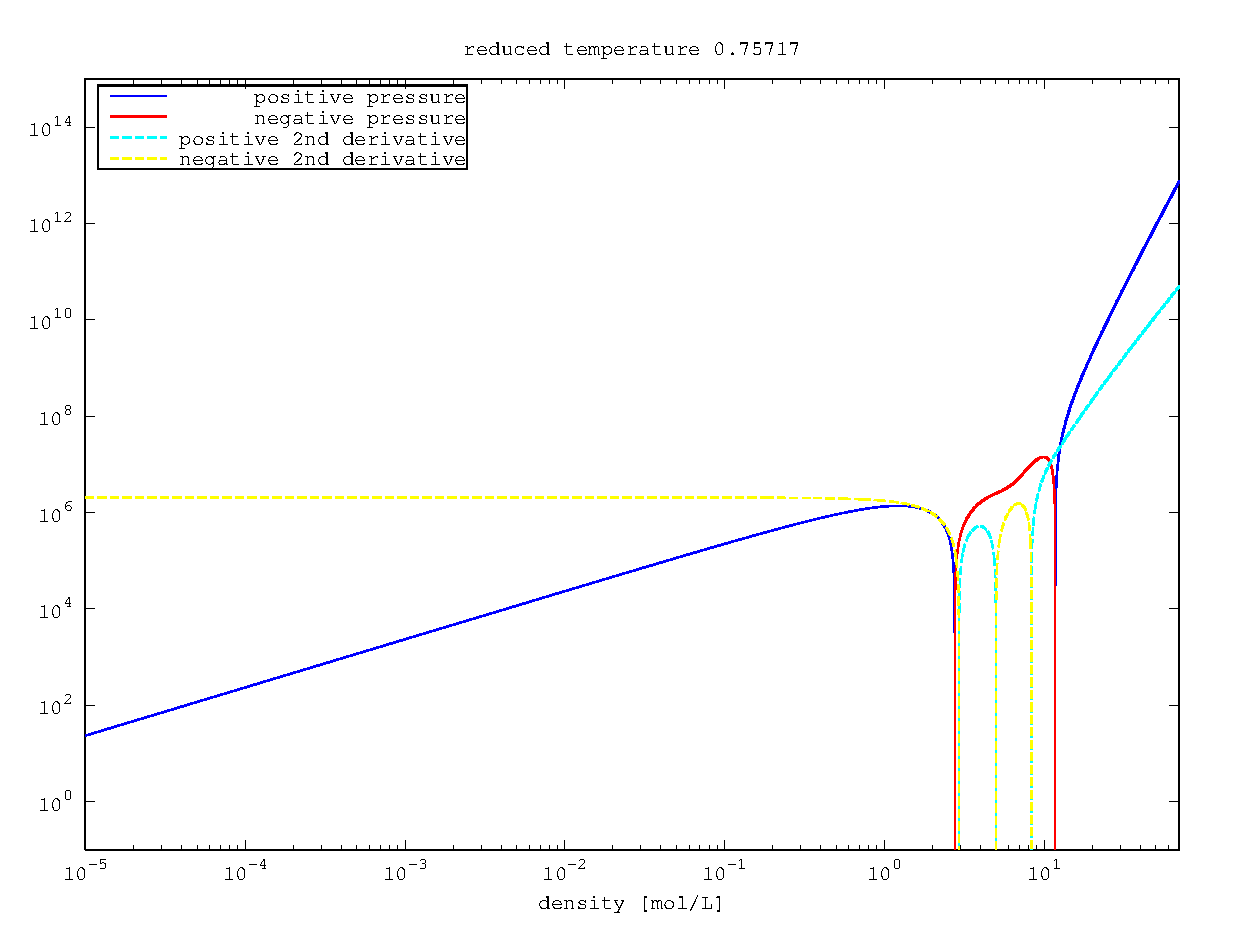
\includegraphics[width=0.7\textwidth]{figures/convexity.eps}
  \caption{A log-log plot of $P(T_0,\rho)$ and $\partial_\rho^2P(T_0,\rho)$ for the MBWR-19 equation with component C$3$.}
  \label{convexityPlot}
\end{figure}
Of course, these convexity properties have not been checked for all
substances in the database. It has been verified to hold for the most
commonly used components, including. C$1$, C$2$, C$3$, N$2$, O$2$,
H$2$O, R$152$a, R$134$a, HE. Moreover, for some components
(e.g. NC$7$, benzene), the vapor hill is only concave for pressures
below the saturated vapor pressure. If these convexity properties
really demonstrate an inherently physical feature of fluids, rather
than simply being numerical artefacts, is not known. E.g. Span
\cite{Span03} seems not to mention anything about convexities. In any
case, let us from now on call the criterion
\begin{equation}
  \partial_\rho^2 P(\rho_{vap},T_0) < 0, \qquad \partial_\rho^2 P(\rho_{liq},T_0) > 0
\end{equation}
the \textbf{phase convexity test}.

Now, by 1. above, we know that if one is looking for a gas root, then
Newton's method will always converge if given an initial density lower
than the true gas density. Similarly, 2. guarantees that Newton's
method converges to the liquid density if the starting density is a
little higher than the true liquid density. 
Of course, this is only true if there really exists a density solution
in the required phase. If not, Newton's method may shoot off. To
prevent this, the density algorithm uses three tests. If the input
phase is vapor, they are:
\begin{enumerate}[i)]
\item $\partial_\rho P(\rho_n) > 0$,
\item $P(\rho_{n-1}) < P(\rho_{n})$,
\item $\lp P(\rho_{n})-P(\rho_{n-1}) \rp / (\rho_{n}-\rho_{n-1})
  < \partial_\rho P(\rho_{n})$.
\end{enumerate}
If the input phase is liquid, they are the same with the exception of
ii, where the direction of the inequality has to be reversed. If the
current iterate fails any of these tests, there is no density root
with the given input phase. Once again, this assumes that the initial
guess is an underestimate in the case of vapor phase, and an overestimate in
the case of liquid phase.

If there exists a vapor root, the solver will always find it when
given vapor as input phase, simply because it is very easy to find a
good underestimate (see section \ref{sec:inDens}). Given liquid as
input phase, a too large overestimate may result in the density solver
diverging. The problem is illustrated in figure \ref{liqGoesDown} for the MBWR-32
equation (this problem does not occur with MBWR-19): if the initial liquid
density is too great, we will have negative slope, and Newton's method
will diverge. To counter this from happening, a fallback Newton solver
is implemented which kicks in if the main density solver fails. The
differences between the fallback Newton solver and the main
solver are two things: the initial liquid guess is lower, and there
are less tests for divergence. In fact, the only situation where the
fallback Newton solver terminates (besides from performing more than
the maximum number of iterations), is when $\partial_\rho P(\rho_n)$
becomes negative.
\begin{figure}[h]
  \centering
  \includegraphics[width=0.7\textwidth]{figures/C3_liqGoesDown.eps}
  \caption{A density-pressure curve for the MBWR-19 equation with
    component C$3$. Note how the computed pressure becomes negative
    for large $\rho$.}
  \label{liqGoesDown}
\end{figure}
A second fallback is also implemented as a last resort, namely the old
solver in TPlib, which is described in section \ref{tplibSolver}.

Finally, some words about the actual code. The density solver is now
divided up into three routines. The routine the user actually calls is
MBWR\_density. MBWR\_density generates initial guesses and then calls
newton\_density, which given an initial density on the correct
side of the root, either determines the root, or outputs $-1$ if no
root is found. An optional argument can force the algorithm to choose
the metastable extremum if no density exists for the input phase; once
again, the routine will only converge if the initial guess is on the
correct side of the density root. If the newton\_density fails, the
function barenewton is called, and if also this fails the TPlib solver
is called.

\subsection{Choosing the initial density} \label{sec:inDens}
As already pointed out, choosing a good initial density is of the utmost
importance for the algorithm to converge to the correct root. For the purposes of reaching the correct density in a robust and time-efficient manner, experimentation showed that the following choices were favorable.

\subsubsection*{Choosing the initial vapor density}
For the vapor root, we use the initial guess 
\begin{itemize}
\item $\rho_{0,\text{vapor}} = 10^{-6}$ if $P \ge 100$ Pa,
\item $\rho_{0,\text{vapor}} = 10^{-12}$ if $P<100$ Pa,
\end{itemize}
This will be lower than the MBWR vapor density (if it exists), just as we desire. Moreover, experiments show that Newton's method converges quickly even though the initial guess is so low. Another advantage of this method of choosing the initial value is that no computation time is spent.

\subsubsection*{Choosing the initial liquid density}
Although one might think that analogously to the choice of initial
vapor density, a really large value (e.g. $10^{2}$
$\mathrm{mol}/\mathrm{L}$) would be a good choice of initial liquid
density, there are two reasons that this is a bad idea. The first is
that unlike in the vapor phase, where the MBWR equation is designed to
have the correct asymptotic behavior $\lim_{\rho \to 0} P(T,\rho) = 0$, one has no guarantee of physical behavior for large $\rho$. Indeed, for MBWR-32, for large enough densities, $P(T,\rho)$ becomes negative. Interestingly and luckily, however, the MBWR-19 equation has a predictable behavior for large $\rho$, namely\footnote{Of course, the two first limits are implied by the last limit.}
$$
\lim_{\rho \to \infty} P_{\text{MBWR-}19}(T,\rho) = \infty,
\quad \lim_{\rho \to \infty} \partial_\rho
P_{\text{MBWR-}19}(T,\rho) = \infty, \quad \lim_{\rho \to \infty} \partial^2_\rho P_{\text{MBWR-}19}(T,\rho) = \infty
$$
No one in the consulted literature seems to mention this, and although it hasn't been checked for all substances in the MBWR-19 database of substances, it holds in all cases we have encountered.

For subcritical temperatures, the density computed by
Soave-Redlich-Kwong is used. For supercritical temperatures, the ideal
gas equation is used. For temperatures and pressures near the critical
point, the critical density is used. In all of these three cases, the
initial density is scaled up by up to $50\%$ or more to ensure that the density is on the right side of the MBWR density. The actual scaling factor varies depending on the situation, guided by experimentation.

\subsection{The density solver in TPlib} \label{tplibSolver}
TPlib uses the second order Newton method, also called Halley's method:
\begin{align*}
  \Delta x_n &= -\frac{f'(x_n)}{f''(x_n)} \pm \frac{1}{f''(x_n)} \sqrt{ f'(x_n)^2 - 2 f''(x_n) (f(x_n)-P) } \\
  &= -\frac{f'(x_n)}{f''(x_n)} \pm \sqrt{ \lp \frac{f'(x_n)}{|f''(x_n)|}
    \rp^2 + 2 \frac{P+f(x_n)}{f''(x_n) } },
\end{align*}
and if the radicand is negative, one sets $\Delta x_n = -f'(x_n) /
f''(x_n)$. 

If the reduced pressure is less than $1$, a so-called Modified Rackett
technique\footnote{See e.g. \cite{GasesAndLiquids01}, section 4.11.} is used to estimate the saturated vapor pressure at the given
temperature, and from this the saturated vapor density can be
estimated. This estimate is then scaled by a factor greater than
$1$.
\begin{align*}
  z_{\mathrm{rackett}} &= (0.29056 - 0.08775\omega)^{1 + (1 - T_r)^{2/7}} \\
  \rho_0 &= \frac{P_c}{R T_c z_{\mathrm{rackett}}}
\end{align*}
For supercritical pressures, the critical density is used
as the initial value. 

The density solver from TPlib has been copied over to the MBWR module
in ThermoPack, with the only modification being that it has been given
the same initial density guess as the main density algorithm. This
reimplementation of the TPlib solver is used to compare the
robustness and computational time with the new density solver. It is
also used as a last fallback routine if the new density algorithm
fails.


\subsection{Testing the density solver robustness}
To optimize and test the density solver, a program which bombards the
density solver with test cases was written. The density solver is
tested for $1000$ equispaced temperatures between the triple point
temperature and $1000$ K; for each of these the pressure input is 1000
equispaced points from the triple point pressure to $10^7$ Pa. This is
done for both the vapor and the liquid phase. All in
all, the density solver is tested on a grid of $2 \cdot 10^6$
points. Our critieria for convergence are
\begin{enumerate}
\item $|P_{MBWR}(\rho)-P_{in}| < 10^{-5}$,
\item $\partial_\rho P_{MBWR}(\rho)> 0$,
\item the phase convexity criterion is fulfilled.
\end{enumerate}
Results from the robustness tests are presented below.

\subsubsection*{MBWR-32}
For the tested components,
\begin{itemize}
\item C1,
\item C2,
\item C3,
\item R134a,
\item O2,
\item N2,
\end{itemize}
the density solver converges in all cases.

\begin{figure}[h]
  \centering
  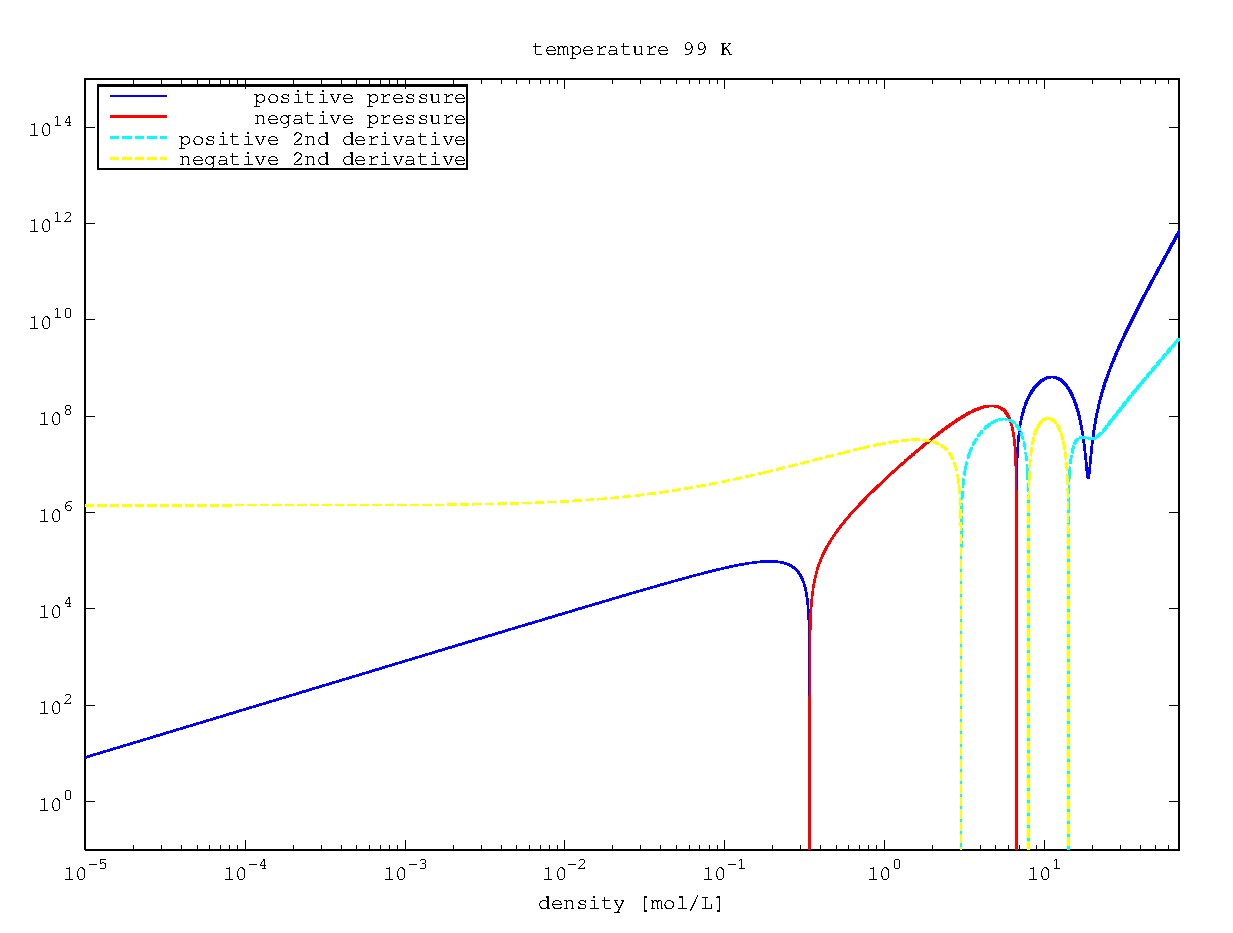
\includegraphics[width=0.6\textwidth]{figures/C2.eps}
  \caption{Density versus pressure for the MBWR-19 equation, component
    C2, temperature $99$ K.}
  \label{C2}
\end{figure}
\begin{figure}[h]
  \centering
  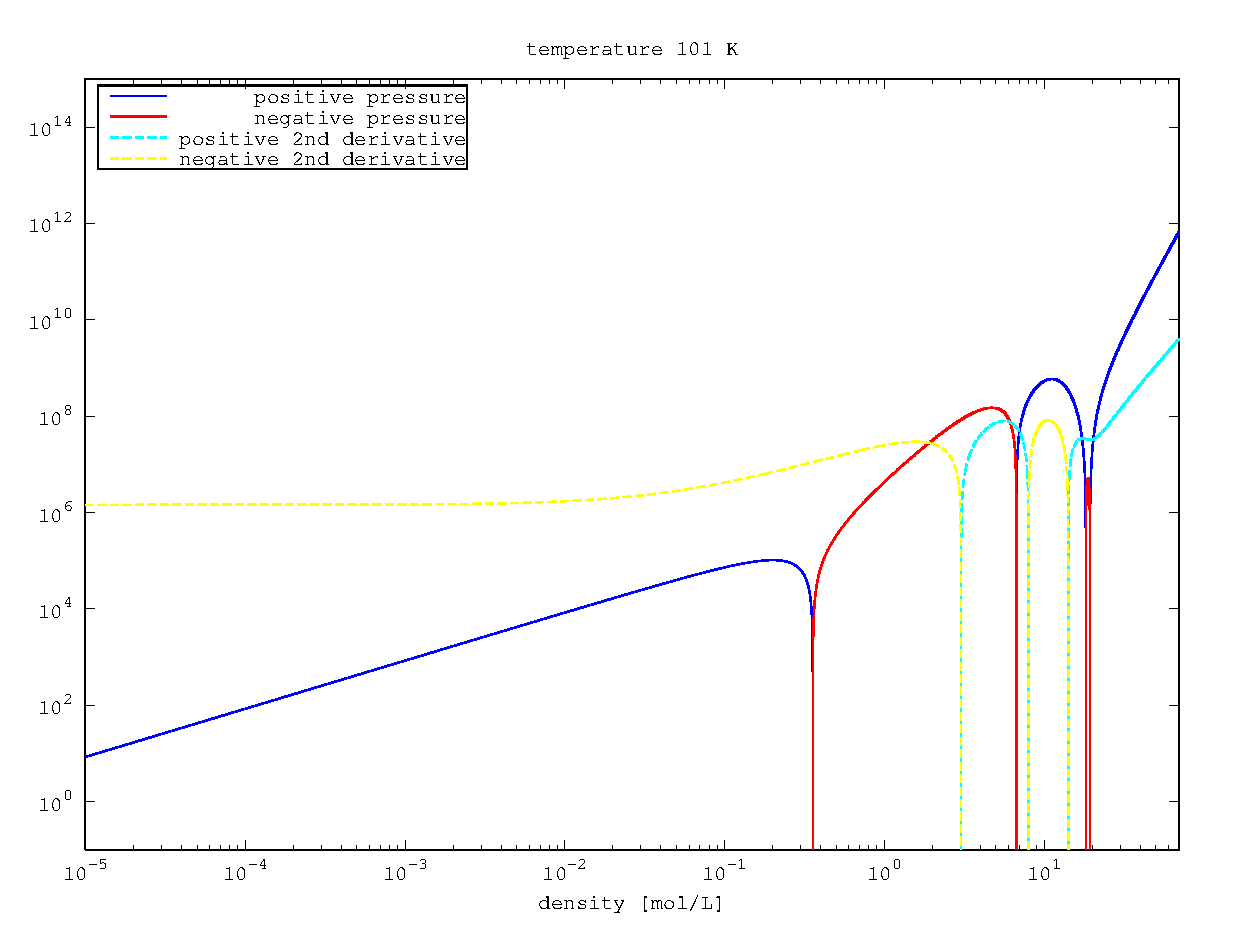
\includegraphics[width=0.6\textwidth]{figures/C2_101.eps}
  \caption{Density versus pressure for the MBWR-19 equation, component
    C2, temperature $101$ K.}
  \label{C2_101}
\end{figure}

\subsubsection*{MBWR-19}
For MBWR-19, we tested 10 components. For the following components the
density solver converges in all cases:
\begin{itemize}
\item C1,
\item C3,
\item O2,
\item N2,
\item R152a,
\item HE,
\item H2O,
\item NH3.
\end{itemize}
We also tested NC7 and C2. As mentioned above, the NC7 vapor hill becomes convex for
pressures higher than the saturated vapor pressure, and therefore some of the
computed vapor densities can fail the phase convexity test. This is
indeed what happens -- 175 failed cases -- when testing the solver and giving
``vapor'' as input phase (using ``liquid'' as input phase always
yields convergence). If one reruns the tests for NC7 while only using
the 1. and 2. convergence criterion, while ignoring the phase
convexity tests, we get attain convergence in all cases.

For C2, the liquid hill looks unusual, see figures \ref{C2} and \ref{C2_101}. These
nonstandard features make it hard for any gradient based solver to
solve for the density, as it requires a very accurate initial density
guess. These problems disappear for temperatures above 100 K, and the
solver then chooses as liquid density the root corresponding to the rightmost
solution; but in this case it is not clear whether this is really the
correct root. In other words, C$2$ seems to be a difficult component
for MBWR-$19$. Although this can be further investigated, and can
probably be remedied by tweaking the solver, this has not been done.

\subsection{Testing the density solver which minimizes the Gibbs energy}
We have also implemented a density algorithm which finds the density
in the phase such that the Gibbs energy is minimized. A quick test using MBWR-19 and water
shows that for $P = 101325$ Pa it changes from having $\rho = 53.2$ mol/L to having $\rho = 0.0331$ mol/L at $373.14$ K. This indeed coincides with the normal boiling point of water.

\subsection{Speed test}
When the MBWR main density routine converges, it is always faster than
the TPlib solver. The speedup depends on the phase, and to a lesser extent on the given temperature and pressure. Typical situations
are shown in Table 3, for various substances and temperature-pressure states. For this table the MBWR-19 equation has been used, and the cpu-time has been measured for $10^5$ calls to the density solver (to render the inherent inaccuracy in the measurement of CPU-time insignificant).

\begin{table}
  \label{MBWR19times}
  \centering
  \begin{tabular}{c c c c c c c c }
    $T$ [K]		        & $P$ [Pa]		& Comp.     & ThermoPack vap. [s] & TPlib vap. [s] & Thermopack liq. [s]  & TPlib liq. [s]  \\
    \hline
    $254$	        & $1.26$e$6$    &$\mathrm C 3$		&$0.14$            & $0.34$	 & $0.11$        &$0.15$	    \\
    $143$               & $2.09$e$6$  	&$\mathrm O2$		&$0.076$           & $0.21$	 & $0.12$     	  &$0.16$		        \\
    $129$	        & $7.46$e$4$   	&$\mathrm{HE}$		&$0.065$           & $0.14$	 & $0.059$    	  &$0.068$		            \\
    $172$               & $5.12$e$5$   	&$\mathrm R152 \mathrm a$	&$0.12$    & $0.27$	 & $0.10$    	  &$0.13$	        \\
    $1000$	        & $1$e$8$      	&$\mathrm C1$ 		&$0.087$            & $0.32$	 & $0.087$    	  &$0.12$	      \\         
  \end{tabular}
  \caption{Performance of the ThermoPack and TPlib density solvers in various circumstances.}
\end{table}

\subsection{Further improvements}
In one sense the density solver converges \textit{too often}; indeed,
it often finds a vapor density even though we are far above the saturated vapor
pressure at the given temperature. Ideally, a correlation for the saturated
vapor pressure should be used in the density routine. This information
could stop the density solver from finding nonexistent roots, and
could further speed up the density solver by terminating the search
when the pressure at the current density iterate is above/below the
saturated vapor pressure (depending on which phase is being solved
for).

\section{Routines for calculating necessary thermodynamic functions}
To get a complete program for the MBWR equations, we have also written
a module for calculating the residual entropy, the residual enthalpy,
the residual Gibbs energy, the $z$-factor and the logarithmic fugacity
coefficients, as well as their first order partial derivatives with
respect to $T$ and $P$. Per now the MBWR equations are only used as a
part of the SPUNG framework, so these thermodynamic functions are
never called. The one exception is the routine for calculating Gibbs
energy, which is used in the in the density routine which chooses the
root having minimal Gibbs energy.


\section{Testing the MBWR models}
To validate the implementation of the MBWR-19 and MBWR-32 models,
various tests have been performed.

\subsection{Thermodynamic identities}
In addition to the numerical test of the derivatives, thermodynamic
identities and identities found from Euler's theorem, serve as decent
consistency tests for the analytical derivatives. The test supplied
here are all found in Michelsen \cite{Michelsen07}. To test the derivatives of the
reduced residual Helmholtz function, the following identities may be
applied:
\begin{align}
  \label{test:1}
  & F = V \pder{F}{V}_{T,\textbf{n}} + \sum_i n_i \pder{F}{n_i}_{T,V} \\
  \label{test:2}
  & V \pdcross{F}{V}{n_i}_T + \sum_j n_j \pdcross{F}{n_j}{n_i}_{T,V} = 0 \\
  \label{test:3}
  & V \pdder{F}{V}_{T,\textbf{n}} + \sum_j n_j \pdcross{F}{n_j}{V}_T =
  0
\end{align}

When these are all satisfied, the fugacity coefficients and their
derivatives may be tested by the identities:
\begin{align}
  \label{test:4}
  & \left( \frac{\partial}{\partial n_j} \sum_i n_i \ln \phi_i \right)_{T,P} = \ln \phi_j \\
  \label{test:5}
  & \pder{\ln \phi_i}{n_j}_{T,P} = \pder{\ln \phi_j}{n_i}_{T,P} \\
  \label{test:6}
  & \sum_i n_i \pder{\ln \phi_i}{n_j}_{T,P} = 0 \\
  \label{test:7}
  & \left( \frac{\partial}{\partial P} \sum_i n_i \ln \phi_i \right)_{T,\textbf{n}} = \frac{(z-1) n}{P} \\
  \label{test:8}
  & \sum_i n_i \pder{ \ln \phi_i}{T}_{P,\textbf{n}} =
  -\frac{H^R(T,P,\textbf{n})}{RT^2}
\end{align}
Of course, since it is an equation for pure substances, the MBWR
equations only has one fugacity
coefficient. All of these identities have been implemented, and the
code seems to fulfill them when tested on a few points.

\subsection{Comparing numerical and analytical derivatives}
The analytical derivatives for the implemented thermodynamic functions
have been compared to their finite-difference counterparts, with
consistent results.

\subsection{Comparison with previous MBWR implementations}
In the code there is an algorithm which calculates the component-specific coefficients for $\alpha(T,P)$ using the component-specific coefficients for $P(T,\rho)$. The coefficents for the Helmholtz energy in the MBWR-32 model with R152a as the substance, checks out with the coefficients computed by an earlier implementation in the NIST thermodynamic library REFPROP.

\section{Extension to mixtures: The SPUNG equation of state}

\subsection{Pure fluid scale factors from a cubic equation of state} % Michelsen p. 102
Consider a generic cubic equation of state,
$$
P = \frac{RT}{v-b}-\frac{a(T)}{(v+\delta_1 b)(v+\delta_2 b)}.
$$
From an equation for $P$, one can find the residual Helmholtz energy from the integral
$A^r(T,V,\mbn) = -\int_\infty^V \lp P - nRT/V' \rp dV'$, and for the
generic cubic equation we
get
\begin{align}
  \frac{A^r(T,v)}{RT} &= -\ln(1-b/v)-\frac{a(T)}{RTb}\frac{1}{\delta_1-\delta_2}\ln \lp \frac{1+\delta_1 b/v}{1+\delta_2 b/v} \rp \\[1.5pt]
  &= -\ln(1-\beta) - \frac{\Gamma}{\delta_1-\delta_2} \ln \lp
  \frac{1+\delta_1 \beta}{1+\delta_2 \beta} \rp, \label{Ar_pure}
\end{align}
where we defined the adimensional parameters $\Gamma = a(T)/bRT$ and
$\beta=b/v$.

We first develop the SPUNG model for pure fluids. Suppose therefore we have two pure fluids called fluid $1$ and fluid $0$. We say they are in \textbf{corresponding states} when $\Gamma_1 =
\Gamma_0$ and $\beta_1 = \beta_0$, i.e. when
\begin{equation}
  \label{Eq:gammaBetaEquality}
  \frac{a_1(T_1)}{b_1 R T_1} = \frac{a_0(T_0)}{b_0 R T_0}, \quad \text{and} \qquad \frac{b_1}{v_1} = \frac{b_0}{v_0}.
\end{equation}
In particular, this implies that the fluids have the same reduced residual Helmholtz energy. Now, for cubic equations of state like PR and SRK, $a(T)$ and $b$ take the special form
\begin{equation}
  \label{aForm}
  a(T) = \Omega_a (R^2T_c^2/P_c) \alpha(T), \quad \alpha(T) =\lp 1+m(\omega)(1-\sqrt{T/T_c}) \rp^2 % THIS LAST SENTENCE ONLY TRUE FOR SRK AND PR? WHICH \omega TO USE FOR MIXTURES?
\end{equation}
and
\begin{equation}
  \label{bForm}
  b = \Omega_b \cdot RT_c/P_c,
\end{equation}
where $\Omega_a$ and $\Omega_b$ are substance-independent constants. From equations \eqref{Eq:gammaBetaEquality} and \eqref{aForm} and \eqref{bForm}, we will be able to calculate the pure
fluid \textbf{scale factors}, defined as
$$
h = v_1/v_0, \qquad f =
T_1/T_0. % These are the definitions for PURE substances, not mixtures! For mixtures, we use the BIG letters \hat H and \hat F.
$$
The scale factor for volume is
\begin{equation}
  \label{eq:h1}
  h = \frac{v_1}{v_0} = \frac{b_1}{b_0} = \frac{T_{c_1}P_{c_0}}{T_{c_0}P_{c_1}},
\end{equation}
while the scale factor for temperature can be written
\begin{equation}
  \label{eq:f1}
  f = \frac{T_1}{T_0} = \frac{a_1(T_1) b_0}{a_0(T_0) b_1} = \frac{T_{c_1}}{T_{c_0}} \frac{\alpha(T_{r_1})}{\alpha(T_{r_0})},
\end{equation}

\subsubsection*{Explicit temperature scale factor when $\alpha=\alpha_{SRK}$ or $\alpha=\alpha_{PR}$}
When the ratio of reduced temperatures, $\theta = T_{r_1}/T_{r_0}$, is
calculated from Soave's or Peng-Robinson's correlation for $\alpha$, we get
\begin{equation}
  \label{theta_1}
  \theta = \lp \frac{1+m_1-m_1 \sqrt{T_{r_1}}}{1+m_0-m_0
    \sqrt{T_{r_0}}} \rp^2,
\end{equation}
It is possible to solve for $\theta_1$ as an explicit function of
$T_{r_1}$. Indeed, taking the square root on both sides of \eqref{theta_1}
and substituting $T_{r_0} = T_{r_1}/\theta$, we get
$$
\sqrt{\theta} = \frac{1+m_1-m_1 \sqrt{T_{r_1}}}{1+m_0-m_0 \sqrt{(T_{r_1}/\theta)} },
$$
and multiplying both sides with the denominator, we can easily solve for $\theta$:
$$
\theta = \lp \frac{1+m_1}{1+m_0} + \frac{m_0-m_1}{1+m_0}
\sqrt{T_{r_1}} \rp^2.
$$
The morale is: when obtaining pure fluid scale factors from cubic equations of
state, one can get explicit expressions for the scale factors,
depending only on the accentric factors and critical parameters, together with the
temperature of one of the substances.

\subsection{Mixtures} % Michelsen p. 105
The most interesting application of SPUNG is when one is dealing with a \textit{mixture} of components, to which we now turn our focus. The idea is to map the thermodynamic state $(T,v)$ for the mixture to some corresponding $(T_0,v_0)$ of a reference fluid. The idea is that if one has a very accurate description (using e.g. a multiparameter equation of state) of the thermodynamics of the pure fluid $0$, then one can use this mapping to get an accurate description of the mixture.

Using a cubic equation, the expression for the Helmholtz energy for
$n$ moles of a mixture is (see e.g. Michelsen \cite[p.105--107]{Michelsen07})
\begin{align*}
  \frac{A_r(T,V,\mbn)}{nRT} &= -\ln(1-B(\mbn)/V)-\frac{D(T,\mbn)}{nRTb}\frac{1}{\delta_1-\delta_2}\ln \lp \frac{1+\delta_1 B(\mbn)/V}{1+\delta_2 B(\mbn)/V} \rp \\[1.5pt]
  &= -\ln(1-\beta_{mix}) - \frac{\Gamma_{mix}}{\delta_1-\delta_2} \ln
  \lp \frac{1+\delta_1 \beta_{mix}}{1+\delta_2 \beta_{mix}} \rp,
\end{align*}
where we have defined the adimensional mixture parameters
as $\Gamma_{mix} = D(T,\mbn)/bRT$ and $\beta_{mix}=B(\mbn)/V$. The quantities
$D(T,\mbn)/n^2$ and $B(\mbn)/n$ are the mixture analogs of the parameters $a(T)$
and $b$ for a pure fluid.

The principle of corresponding states allows us to calculate the
reduced residual energy of a mixture from the reduced residual
Helmholtz energy of a pure reference fluid $0$, by equating $\Gamma_{mix} =
\Gamma_0$ and $\beta_{mix} = \beta_0$, i.e.
$$
\frac{D(T,\mbn)}{nRTB(\mbn)} = \frac{a_0(T_0)}{RT_0b_0} \qquad \text{and} \qquad
\frac{B(\mbn)}{V} = \frac{b_0}{v_0}.
$$
We thus get the two mixture scale factors $\hat H$ and $\hat F$
$$
\hat H = \frac{V}{v_0} = \frac{B(\mbn)}{b_0}, \qquad \text{and} \qquad \hat
F = \frac{nT}{T_0} = \frac{D(T,\mbn)}{B(\mbn)} \frac{b_0}{a_0(T_0)}.
$$
Note that the mixture scale factors are first order homogeneous
functions in the mole numbers. The mixing rules
adopted for $B(\mbn)$ and $D(T,\mbn)$ are optional as long as they give a consistent
model. %The mixing rules for $\hat H$ and $\hat F$ are derived from the mixing rules for $D$ and $B$.

Adopting the conventional mixing rules -- also called the van der Waals
one-fluid mixing rules, or the quadratic mixing rules -- for $B(\mbn)$ and $D(T,\mbn)$, we get
$$
\hat H n b_0 = nB(\mbn) = \sum_{i,j} n_i n_j b_{ij}
$$
and
$$
\hat F \hat H a_0(T_0) = \hat F \hat H a_0(nT/\hat F) = D(T,\mbn) = \sum_{i,j}
n_i n_j a_{ij}(T).
$$
For mixtures involving polar substances, mixture rules based on excess
Gibbs energy models may be more appropriate. The Huron-Vidal mixing
rule is a prominent example. We mention that the cubic equation of state which is used to calculate the scale
factors $\hH$ and $\hF$ is called the \textbf{scale factor equation}
or the \textbf{shape factor equation}. $\hH$ and $\hF$ are often
called shape factors.

Although $\hH$ is given explicitly in terms of the mixture composition
as $\hat H = \frac{B(\mbn)}{b_0}$, it is in the general case
impossible to give an explicit expression for $\hF$ in terms of the
mixture temperature and composition. In certain cases however, this
can be done.

\subsubsection*{Explicit temperature scale factor when $\alpha=\alpha_{SRK}$ or $\alpha=\alpha_{PR}$}
If $a_0(T_0) = a_{0c} (1+m_0-m_0 \sqrt{T_0/T_{0c}})^2$, it
turns out that we can solve for $\hF$ from the implicit expression
$$
\hat F =  \frac{1}{\hH} \frac{D(T,\mbn)}{a_0(nT/\hF)}.
$$
Indeed, by inserting the form for $a_0$ we get
$$
\hat F = \frac{D(T,\mbn)}{\hH a_{0c} \lp 1+m_0-m_0 \sqrt{nT/(\hF T_{0c})} \rp^2}
$$
$$
\sqrt{\hat F} \lp 1+m_0-m_0 \sqrt{\frac{nT}{\hF T_{0c}}}\rp = \lp
\frac{D(T,\mbn)}{\hH a_{0c}} \rp^{1/2}
$$
$$
\sqrt{\hat F} (1+m_0) = m_0 \sqrt{\frac{nT}{T_{0c}}} +  \lp
\frac{D(T,\mbn)}{\hH a_{0c}} \rp^{1/2}
$$
\begin{equation}
  \label{hF_SRK}
  \hat F = \frac{1}{(1+m_0)^2}\lp m_0 \sqrt{\frac{nT}{T_{0c}}} + \lp
  \frac{D(T,\mbn)}{\hH a_{0c}} \rp^{1/2} \rp^2.
\end{equation}

\subsubsection*{Temperature scale factor when $\alpha=\alpha_{TWU}$}
Suppose now that we use the alpha formulation of Twu-Coon-Cunningham:
$$
a_0(T_0) = a_{0c} \cdot T_{0r}^{N(M-1)} \exp \lp L - LT_{0r}^{MN} \rp,
$$
where the $L$, $M$ and $N$ have been fitted to vapor pressure data for
each fluid. This alpha correlation is more tailored to specific
components than $\alpha_{SRK}$ , seeing as the only component-specific
input to $\alpha_{SRK}$ is the acentric factor and the critical
temperature. In the current database the parameters have only been
stored for the four substances $\mathrm{CO}_2$, $\mathrm{CH}_4$,
$\mathrm{H}_2\mathrm{S}$ and $\mathrm{H}_2\mathrm{O}$.

Let us find the temperature shape factor using this alpha
formulation. Using $\hat F = \frac{D(T,\mbn)}{\hH
  a_{0c}\alpha_{TWU}(T_0)}$ and $T_0 = nT/\hF$, we get
$$
\hat F \cdot \lp \frac{nT}{\hF T_{0c}} \rp^{N(M-1)} \exp \lp L - L\lp \frac{nT}{\hF T_{0c}} \rp^{MN} \rp = \frac{D(T,\mbn)}{\hH
  a_{0c}},
$$
or
\begin{equation}
  \label{hF_TWU}
  \hF^{1+N(1-M)} \exp \lp L - L\lp \frac{nT}{\hF T_{0c}} \rp^{MN} \rp =
  \lp \frac{T_{0c}}{nT} \rp^{N(M-1)} \frac{D(T,\mbn)}{\hH a_{0c}}.
\end{equation}
From this last expression, it is clear that it is not possible to
solve for $\hF$ using simple functions\footnote{It is solvable by
  using the Lambert W function, but this transcendental function is
  not available from the numerical libraries used by ThermoPack.}.
The code therefore solves this using Newton's method, with the $\hF$
factor computed with $\alpha_{SRK}$, \eqref{hF_SRK}, as starting value.

A drawback is that these coefficients are only valid for subcritical
temperatures $T_{0r}<1$. Skaugen \cite{Skaugen13} gives a
more detailed discussion of the Twu correlation, and what can be done
for supercritical temperatures.

Finally, we point out that if one wants to implement other
$\alpha$-formulations into the SPUNG code, this is straightforward as
one can simply mirror the code for $\alpha_{SRK}$ (if an explicit
expression for $\hF$ is available) or $\alpha_{TWU}$ (if $\hF$ has to
be solved iteratively). 

\subsection{Partial derivatives} % Michelsen, p. 115.
We now calculate partial derivatives in the case where we use a cubic
equation to compute the shape factors, and where we use the
conventional mixing rules for $D$ and $B$. Note that they choice of
$\alpha$ in the cubic equation can be anything.

Let us sum up the relevant formulas once more. The principle of
corresponding states tells us that given a mixture in the state
$(T,V,\mbn)$, we have that
\begin{equation}
  A^r(T,V,\mbn) = \hat F M(T_0,v_0),
\end{equation}
where $(T_0,v_0)$ is the reference state, defined as
\begin{equation}
  v_0 = \frac{V}{\hat H}, \qquad T_0 = \frac{nT}{\hat F},
\end{equation}
where the scale factors $\hat H$ and $\hat F$ are given by
\begin{equation}
  \hat H = \frac{B}{b_0}, \qquad \hat F = \frac{D}{B} \frac{b_0}{a_0(T_0)}.
\end{equation}
Here $D$ and $B$ given by the van der Waals mixing rule
\begin{equation}
  nB = \sum_{i} n_i \sum_j n_j b_{ij}
\end{equation}
\begin{equation}
  D = \sum_{i} n_i \sum_j n_j a_{ij}(T)
\end{equation}
$B(\mbn)$ and $D$ are completely determined from the underlying cubic
equation of state.

We again stress the point that $\hH = \hH(\mbn)$ only depends on
composition, while $\hF = \hF(T,\mbn)$ only depends on temperature and
composition.

First we calculate the first and second order partial derivatives of
$A^r(T,V,\mbn)$ with respect to $T$, $V$ and $n_i$ in terms of the
partial derivatives of $\hH$ and $M$ with respect to $T$, $V$ and
$n_i$.
\begin{align}
  \pdersub{A^r}{T}{V,\mbn} &= \hF_TM+\hF M_T \\
  \pdersub{A^r}{V}{T,\mbn} &= \hF M_V \\
  \pdersub{A^r}{n_i}{T,V} &= \hF_iM + \hF M_i \\
  \pddersub{A^r}{T}{V,\mbn} &= \hF_{TT}M + 2\hF_TM_T + \hF M_{TT} \\
  \pddersub{A^r}{V}{T,\mbn} &= \hF M_{VV} \\
  \pdcrosssub{A^r}{n_i}{n_j}{T,V} &= \hF_{ij}M + \hF_i M_j + \hF_j M_i + \hF M_{ij} \\
  \pdcrosssub{A^r}{T}{V}{\mbn} &= \hF_TM_V+\hF M_{TV} \\
  \pdcrosssub{A^r}{T}{n_i}{V} &= \hF_{Ti}M + \hF_i M_T + \hF_T M_i + \hF M_{Ti} \\
  \pdcrosssub{A^r}{V}{n_i}{T} &= \hF_i M_V + \hF M_{Vi}
\end{align}
Next we calculate the first and second order partial derivatives of
$M$ with respect to $T$, $V$ and $n_i$ in terms of the partial
derivatives of $M$ with respect to $T_0$, $v_0$ and the derivatives of
$T_0$ and $v_0$ with respect to $T$, $V$ and $n_i$.
\begin{align} % Double-check these.
  M_T    &= M_{T_0}T_{0,T} \\
  M_V    &= M_{v_0}v_{0,V} \\
  M_i    &= M_{T_0}T_{0,i} + M_{v_0}v_{0,i} \\
  M_{TT}  &= M_{T_0T_0}T_{0,T}^2 + M_{T_0}T_{0,TT} \\
  M_{VV}  &= M_{v_0v_0}v_{0,V}^2 + M_{v_0}v_{0,VV} \\
  M_{ij}  &= M_{T_0T_0}T_{0,i}T_{0,j} + M_{T_0}T_{0,ij} + M_{v_0v_0}v_{0,i}v_{0,j} \\
  &+ M_{v_0}v_{0,ij} + M_{T_0v_0}(T_{0,i}v_{0,j}+T_{0,j}v_{0,i}) \\
  M_{TV}  &= M_{T_0v_0}T_{0,T}v_{0,V} \\
  M_{Ti}  &= M_{T_0T_0}T_{0,T}T_{0,i} + M_{T_0v_0} T_{0,T} v_{0,i} + M_{T_0}T_{0,Ti} \\
  M_{Vi} &= M_{v_0v_0}v_{0,V}v_{0,i} + M_{T_0v_0} T_{0,i} v_{0,V} +
  M_{v_0}v_{0,Vi}
\end{align}
\subsection*{Partial derivatives of $B$ with respect to $\mbn$}
$$
B_i = \frac{\partial}{\partial n_i} \lp \frac{\sum_i \sum_j n_i n_j
  b_{ij}}{n} \rp = \frac{\lp 2 \sum_j n_j b_{ij} \rp n - \sum_i \sum_j
  n_i n_j b_{ij}}{n^2} = \frac{2 \sum_j n_j b_{ij} -B}{n}
$$
$$
B_{ij} = \frac{\partial^2}{\partial n_i \partial n_j} \lp \frac{2
  \sum_k n_k b_{ik} -B}{n} \rp = \frac{\lp 2b_{ij}-B_j \rp n - \lp 2
  \sum_k n_k b_{ik} -B \rp}{n^2} = \frac{2b_{ij}-B_i-B_j}{n}
$$
\subsection*{Partial derivatives of $\hH$ with respect to $\mbn$}
We can get the partial derivatives of $\hH$ can be written in terms of
the partial derivatives of $B$:
\begin{equation}
  \hH_i = \frac{B_i}{b_0} = \frac{2 \sum_j n_j b_{ij} -B}{nb_0}
\end{equation}
\begin{equation}
  \hH_{ij} = \frac{B_{ij}}{b_0} = \frac{2b_{ij}-B_i-B_j}{nb_0}
\end{equation}
\subsection*{Partial derivatives of $v_0$ with respect to $V$ and
  $\mbn$}
We now find the partial derivatives of $v_0$. To find the derivatives
with respect to composition, we use $\hH v_0 = V$ to get
$$
\hH_i v_0 + \hH v_{0,i} = 0, \qquad \hH_{ij} v_0 + \hH_i v_{0,j} +
\hH_j v_{0,i} + \hH v_{0,ij} = 0.
$$
Thus
\begin{equation}
  \frac{v_{0,i}}{v_0} = - \frac{\hH_i}{\hH} = - \frac{B_i}{B},
\end{equation}
and
\begin{equation}
  \frac{v_{0,ij}}{v_0} = -\frac{\hH_{ij}}{\hH} - \frac{\hH_i}{\hH} \frac{v_{0,j}}{v_0} - \frac{\hH_j}{\hH} \frac{v_{0,i}}{v_0} = -\frac{B_{ij}}{B} + 2 \frac{B_i}{B} \frac{B_j}{B}
\end{equation}
The $V$-derivatives of $v_0$ can be found by differentiating $\hH v_0
= V$ with respect to $V$. This gives
\begin{align}
  v_{0,V}  &= \frac{1}{\hH} \\
  v_{0,VV} &= 0 \\
  v_{0,Vi} &= -\frac{\hH_i}{\hH^2} = -\frac{B_i b_0}{B^2}
\end{align}
\subsection*{Partial derivatives of $T_0$ with respect to $T$ and
  $\mbn$}
To find the derivatives with respect to composition, we use $\hF T_0 =
nT$ to get
$$
\hF_i T_0 + \hF T_{0,i} = T, \qquad \hF_{ij} T_0 + \hF_i T_{0,j} +
\hF_j T_{0,i} + \hF T_{0,ij} = 0.
$$
Thus
\begin{equation}
  \label{T_0i}
  \frac{T_{0,i}}{T_0} = \frac{T}{\hF T_0}- \frac{\hF_i}{\hF} = \frac1n - \frac{\hF_i}{\hF},
\end{equation}
and similarly we find
\begin{equation}
  \frac{T_{0,T}}{T_0} = \frac{1}{T} - \frac{\hF_T}{\hF}
\end{equation}
The second order partials are given by
\begin{align}
  \frac{T_{0,ij}}{T_0} &= -\frac{\hF_{ij}}{\hF} - \frac{\hF_i}{\hF} \frac{T_{0,j}}{T_0} - \frac{\hF_j}{\hF} \frac{T_{0,i}}{T_0}, \label{T_0ij} \\
  \frac{T_{0,Ti}}{T_0} &= -\frac{\hF_{Ti}}{\hF} - \frac{\hF_i}{\hF}
  \frac{T_{0,T}}{T_0} - \frac{\hF_T}{\hF} \frac{T_{0,i}}{T_0} + \frac{1}{\hF} \label{T_0Ti} \\
  \frac{T_{0,TT}}{T_0} &= -\frac{\hF_{TT}}{\hF} - 2\frac{\hF_T}{\hF}
  \frac{T_{0,T}}{T_0}. \label{T_0TT}
\end{align}
Note that Michelsen \cite{Michelsen07} has an error in the expression
for $T_{0,Ti}/T_0$, as the last term on the right hand side is missing.
\subsection*{Partial derivatives of $D$ with respect to $T$ and
  $\mbn$}
\begin{align}
  D_i   &= 2 \sum_j n_j a_{ij} \\
  D_{iT} &= 2 \sum_j n_j \lp \partial a_{ij}/\partial T \rp \\
  D_{ij} &= 2a_{ij} \\
  D_{T}  &= \tfrac12 \sum_i n_i D_{iT} \\
  D_{TT} &= \sum_i n_i \sum_j n_j \lp \partial^2 a_{ij}/\partial T^2
  \rp
\end{align}
\subsection*{Partial derivatives of $\hF$ with respect to $T$ and
  $\mbn$}
We now calculate the partial derivatives for $\hF$ with respect to
temperature and composition in terms of the partial derivatives of
$D$, $\hH$ and $a_0$. To do this differentiate $\hF(T,\mbn) \hH(\mbn)
a_0(T_0) = D(T,\mbn)$ with respect to composition, giving
$$
\hF_i \hH a_0 + \hF \hH_i a_0 + \hF \hH a_{0,T_0} T_{0,i} = D_i = 2
\sum_j n_j a_{ij},
$$
which when divided by $D = \hF \hH a_0$ becomes
$$
\frac{\hF_i}{\hF} + \frac{\hH_i}{\hH} +
\frac{a_{0,T_0}}{a_{T_0}}T_{0,i}= \frac{D_i}{D}.
$$
By using the expression \eqref{T_0i} to eliminate $T_{0,i}$, we end up
with
$$
\frac{\hF_i}{\hF} \lp 1-\frac{a_{0,T_0}}{a_0} T_0 \rp +
\frac{\hH_i}{\hH} + \frac{a_{0,T_0}}{a_{T_0}}\frac{T_0}{n} =
\frac{D_i}{D},
$$
and thus
\begin{equation}
  \frac{\hF_i}{\hF} = \frac{\frac{D_i}{D} - \frac{B_i}{B} - \frac{a_{0,T_0}}{a_{T_0}}\frac{T_0}{n}}{1-\frac{a_{0,T_0}}{a_0} T_0}.
\end{equation}
Similarly, we find
\begin{equation}
  \frac{\hF_T}{\hF} = \frac{\frac{D_T}{D} - \frac{a_{0,T_0}}{a_{T_0}}\frac{T_0}{T}}{1-\frac{a_{0,T_0}}{a_0} T_0}.
\end{equation}
To derive the second order partial derivative of $\hF$ with respect to
composition we differentiate $\hF(T,\mbn) \hH(\mbn) a_0(T_0) =
D(T,\mbn)$ twice. This gives
\begin{align*}
  &\hF_{ij} \hH a_0 + \hF_i \hH_j a_0 + \hF_i\hH a_{0,T_0} T_{0,j} + \\
  &\hF_{j} \hH_i a_0 + \hF \hH_{ij} a_0 + \hF \hH_i a_{0,T_0} T_{0,j} + \\
  &\hF_j \hH a_{0,T_0} T_{0,i} + \hF \hH_j a_{0,T_0} T_{0,i} + \hF \hH
  (a_{0,T_0T_0} T_{0,i} T_{0,j} + a_{0,T_0} T_{0,ij}) = 2 a_{ij},
\end{align*}
and dividing by $D = \hF \hH a_0$, we get the cleaner expression
\begin{equation}
  \label{hF_ij}
  \begin{aligned}
    &\frac{\hF_{ij}}{\hF} + \frac{\hF_i}{\hF}\frac{\hH_j}{\hH} + \frac{\hF_i}{\hF}\frac{a_{0,T_0}}{a_0} T_{0,j} + \\
    &\frac{\hF_{j}}{\hF} \frac{\hH_i}{\hH} + \frac{\hH_{ij}}{\hH} + \frac{\hH_i}{\hH}\frac{a_{0,T_0}}{a_0} T_{0,j} + \\
    &\frac{\hF_j}{\hF}\frac{a_{0,T_0}}{a_0} T_{0,i} +
    \frac{\hH_j}{\hH}\frac{a_{0,T_0}}{a_0} T_{0,i} +
    \frac{a_{0,T_0T_0}}{a_0} T_{0,i} T_{0,j} + \frac{a_{0,T_0}}{a_0}
    T_{0,ij} = \frac{D_{ij}}{D}.
  \end{aligned}
\end{equation}
We similarly get
\begin{equation}
  \label{hF_Ti}
  \begin{aligned}
    &\frac{\hF_{Ti}}{\hF} + \frac{\hF_i}{\hF}\frac{a_{0,T_0}}{a_0} T_{0,T} + \\
    &\frac{\hF_{T}}{\hF} \frac{\hH_i}{\hH} + \frac{\hH_i}{\hH}\frac{a_{0,T_0}}{a_0} T_{0,T} + \\
    &\frac{\hF_T}{\hF}\frac{a_{0,T_0}}{a_0} T_{0,i} +
    \frac{a_{0,T_0T_0}}{a_0} T_{0,i} T_{0,T} + \frac{a_{0,T_0}}{a_0}
    T_{0,Ti} = \frac{D_{Ti}}{D},
  \end{aligned}
\end{equation}
and
\begin{equation}
  \label{hF_TT}
  \frac{\hF_{TT}}{\hF} + \frac{2\hF_T}{\hF}\frac{a_{0,T_0}}{a_0} T_{0,T} + \frac{a_{0,T_0T_0}}{a_0} (T_{0,T})^2 + \frac{a_{0,T_0}}{a_0} T_{0,TT} = \frac{D_{TT}}{D}.
\end{equation}
% By using equations \eqref{T_0ij}, \eqref{T_0Ti} and \eqref{T_0TT},
% we eliminate the derivatives of $T_0$ in the expressions
% \eqref{hF_ij}, \eqref{hF_Ti} and \eqref{hF_TT}, giving
% us % for $\hF_{ij}$, $\hF_{iT}$ and $\hF_{TT}$.
By substituting the expression for $T_{0,ij}$ into \eqref{hF_ij}, we
get
\begin{align*}
  &\frac{\hF_{ij}}{\hF} + \frac{\hF_i}{\hF}\frac{\hH_j}{\hH} + \frac{\hF_i}{\hF}\frac{a_{0,T_0}}{a_0} T_{0,j} + \\
  &\frac{\hF_{j}}{\hF} \frac{\hH_i}{\hH} + \frac{\hH_{ij}}{\hH} + \frac{\hH_i}{\hH}\frac{a_{0,T_0}}{a_0} T_{0,j} + \\
  &\frac{\hF_j}{\hF}\frac{a_{0,T_0}}{a_0} T_{0,i} +
  \frac{\hH_j}{\hH}\frac{a_{0,T_0}}{a_0} T_{0,i} +
  \frac{a_{0,T_0T_0}}{a_0} T_{0,i} T_{0,j} + \frac{a_{0,T_0}}{a_0} \lp
  -\frac{\hF_{ij}}{\hF} T_0 - \frac{\hF_i}{\hF} T_{0,j} -
  \frac{\hF_j}{\hF} T_{0,i} \rp = \frac{D_{ij}}{D},
\end{align*}
and thus
\begin{equation}
  \begin{aligned}
    \frac{\hF_{ij}}{\hF} =& \frac{ \frac{D_{ij}}{D} - \frac{\hF_i}{\hF}\frac{\hH_j}{\hH} - \frac{\hF_{j}}{\hF} \frac{\hH_i}{\hH} - \frac{\hH_{ij}}{\hH} }{1-\frac{a_{0,T_0}}{a_0} T_0} \\
    +& \frac{-\frac{\hH_j}{\hH}\frac{a_{0,T_0}}{a_0} T_{0,i} -
      \frac{\hH_i}{\hH}\frac{a_{0,T_0}}{a_0} T_{0,j} -
      \frac{a_{0,T_0T_0}}{a_0} T_{0,i}
      T_{0,j}}{1-\frac{a_{0,T_0}}{a_0} T_0}.
  \end{aligned}
\end{equation}
We also get\footnote{Michelsen \cite{Michelsen07} has an error in the
  expression for $\hF_{Ti}/\hF$: he is missing the last term in
  the numerator.}
\begin{equation}
  \begin{aligned}
    \frac{\hF_{Ti}}{\hF} =& \frac{ \frac{D_{iT}}{D} -
      \frac{\hF_{T}}{\hF} \frac{\hH_i}{\hH} -
      \frac{\hH_i}{\hH}\frac{a_{0,T_0}}{a_0} T_{0,T} -
      \frac{a_{0,T_0T_0}}{a_0} T_{0,i} T_{0,T} - \frac{a_{0,T_0}}{a_0 \hF}}{1-\frac{a_{0,T_0}}{a_0} T_0}.
  \end{aligned}
\end{equation}
and
\begin{equation}
  \begin{aligned}
    \frac{\hF_{TT}}{\hF} =& \frac{ \frac{D_{TT}}{D} -
      \frac{a_{0,T_0T_0}}{a_0} (T_{0,T})^2}{1-\frac{a_{0,T_0}}{a_0}
      T_0}.
  \end{aligned}
\end{equation}

\subsubsection*{Relationship between $P_0$ and $P$}
In general, we have
$$
P = -\pdersub{A^r}{V}{T,\mbn} + \frac{nRT}{V}.
$$
Using that $A^r(T,V,\mbn) = \hF M(T_0,v_0)$ we get
\begin{align*}
  P &= -\partial_V \lp \hF(T,\mbn) M(T_0,v_0) \rp + \frac{RT}{v} \\
  &= -\hF M_{v_0} v_{0,V} + \frac{nR(\hF T_0/n)}{\hH v_0} \\
  &= \frac{\hF}{\hH} \lp -M_{v_0} + \frac{RT_0}{v_0} \rp \\
  &= \frac{\hF}{\hH} P_0.
\end{align*}

\subsubsection*{Expressing $F$ in terms of $M$}
Often we are more interested in the reduced residual Helmholtz energy
$F(T,V,\mbn) = A^r(T,V,\mbn)/RT$ than in $A^r(T,V,\mbn)$ itself. First
note that since $\hF = nT/T_0$ we get that $A^r(T,V,\mbn) = \hF
M(T_0,v_0)$ is equivalent with
$$
F(T,V,\mbn) = \frac{n}{RT_0} M(T_0,v_0).
$$
\begin{align}
  \pdersub{F}{T}{V,\mbn} &= -\frac{n}{RT_0^2} T_{0,T} M +\frac{n}{RT_0} M_T \\
  \pdersub{F}{V}{T,\mbn} &= \frac{n}{RT_0} M_V \\
  \pdersub{F}{n_i}{T,V} &= \lp \frac{1}{RT_0} - \frac{n}{RT_0^2} T_{0,i} \rp M + \frac{n}{RT_0} M_i \\
  \pddersub{F}{V}{T,\mbn} &= \frac{n}{RT_0} M_{VV} \\
  \pdcrosssub{F}{T}{V}{\mbn} &= -\frac{n}{RT_0^2} T_{0,T} M_V +\frac{n}{RT_0} M_{TV} \\
  \pdcrosssub{F}{V}{n_i}{T} &= \lp \frac{1}{RT_0} - \frac{n}{RT_0^2} T_{0,i} \rp M_V + \frac{n}{RT_0} M_{Vi} \\
  \pddersub{F}{T}{V,\mbn} &= \lp \frac{2n}{RT_0^3} T_{0,T}^2 -
  \frac{n}{RT_0^2} T_{0,TT} \rp M - \frac{2n}{RT_0^2} T_{0,T} M_T +
  \frac{n}{RT_0} M_{TT}
\end{align}
\begin{align}
  &\begin{aligned}
    \pdcrosssub{F}{n_i}{n_j}{T,V} &= \lp -\frac{1}{RT_0^2} T_{0,j} - \frac{1}{RT_0^2} T_{0,i} + \frac{2n}{RT_0^3} T_{0,i} T_{0,j} - \frac{n}{RT_0^2} T_{0,ij} \rp M \\
    &+ \lp \frac{1}{RT_0} - \frac{n}{RT_0^2} T_{0,i} \rp M_j + \lp \frac{1}{RT_0} - \frac{n}{RT_0^2} T_{0,j} \rp M_i + \frac{n}{RT_0} M_{ij} \\
  \end{aligned} \\
  &\begin{aligned}
    \pdcrosssub{F}{T}{n_i}{V} &= \lp -\frac{1}{RT_0^2} T_{0,T} + \frac{2n}{RT_0^3} T_{0,i} T_{0,T} - \frac{n}{RT_0^2} T_{0,Ti} \rp M \\
    &+ \lp \frac{1}{RT_0} - \frac{n}{RT_0^2} T_{0,i} \rp M_T -
    \frac{n}{RT_0^2} T_{0,T} M_i + \frac{n}{RT_0} M_{Ti}
  \end{aligned}
\end{align}

\section{Testing the SPUNG model}
To validate the implementation of the SPUNG model, various tests have
been performed.

\subsection{Equivalence of cubic equations vs SPUNG with cubic reference
  equation}
Using SPUNG with SRK as both shape factor equation and reference
equation should be equivalent to using SRK directly. It is readily
checked that this is indeed the for the ThermoPack SPUNG implementation.

\subsection{Computing phase envelopes}
We compare the performance of the ThermoPack SPUNG model against
the TPlib SPUNG model, as well as experimental measurements. We use
SRK as the shape equation and MBWR-32 as the reference equation The
mixture we consider consists of $\mathrm{CO}_2$ and $\mathrm N_2$ at
fixed temperature $T=240 \, \mathrm{K}$. The results are shown in
Figure \ref{fig:phaseEnv}.

\begin{figure}[h]
  \centering
  \includegraphics[width=0.7\textwidth]{figures/phaseEnvelope_regular.pdf}
  \caption{Computed and measured points on the phase envelope for the mixture
    $\mathrm{CO}_2-\mathrm N_2$ at $T=240 \, \mathrm{K}$.}
  \label{fig:phaseEnv}
\end{figure}

The reason why there are no TPlib points on the top of the graph is
that the TPlib SPUNG model is not able to close the envelope. This
demonstrates the improved robustness of the ThermoPack library
compared to TPlib.

Since the model is the same in TPlib and ThermoPack, the computed
points for TPlib should lie exactly on the computed curve for
ThermoPack. This is clearly not the case in Figure
\ref{fig:phaseEnv}. The reason for this is that in TPlib there is a database of interaction
parameters $k_{ij}$ that have been optimized for the SPUNG model. They
are given for SRK, SRK-GD and PR, and for a range of mixtures. In
Figure \ref{fig:phaseEnv_opt} we have plotted the same curve as in
Figure \ref{fig:phaseEnv}, but using the optimized interaction
parameters in ThermoPack.
\begin{figure}[h]
  \centering
  \includegraphics[width=0.7\textwidth]{figures/phaseEnvelope_optimized.pdf}
  \caption{The $\mathrm{CO}_2-\mathrm N_2$ phase envelope using
    optimized interaction parameters.}
  \label{fig:phaseEnv_opt}
\end{figure}
The TPlib points fit perfectly, except one point (the second point
from the left) which is an almost perfect match with with the
experimental measurement. The reason for this one anomaly is
unknown. Fortunately, we have experimental data also for CO$_2$-O$_2$,
and Figures \ref{fig:O2reg} and \ref{fig:O2opt} show that the
ThermoPack implementation is consistent with the TPlib
implementation. How much the optimized interaction parameters actually
improve the fit, is not known.

\begin{figure}[h]
  \centering
  \includegraphics[width=0.7\textwidth]{figures/phaseEnvelope_O2_regular.pdf}
  \caption{The $\mathrm{CO}_2-\mathrm O_2$ phase envelope using
    regular interaction parameters.}
  \label{fig:O2reg}
\end{figure}

\begin{figure}[h]
  \centering
  \includegraphics[width=0.7\textwidth]{figures/phaseEnvelope_O2_optimized.pdf}
  \caption{The $\mathrm{CO}_2-\mathrm O_2$ phase envelope using
    optimized interaction parameters.}
  \label{fig:O2opt}
\end{figure}

\subsection{Comparing with density measurements}
We compare density measurements for a mixture of $98$ \% CO$_2$ and $2$ \% CH$_4$ with three models: standard SRK, and SPUNG-SRK with CH$_4$ as reference component, and using respectively MBWR-19 and MBWR-32 as reference equation. The measurements are in the pressure range $2\cdot 10^6 -- 3.5 \cdot 10^7$ Pa, and the temperature range $225--350$ K. In Figure \ref{SRK_density} we have plotted the deviation from the measurements (the line) and the results using SRK (the points). There are two outliers, which is probably due to the SRK density solver choosing the wrong phase. To avoid this from happening to the SPUNG calculations, the density solver which minimizes Gibbs energy was invoked when the density for the reference component was computed. The results for the SPUNG models are shown in Figure \ref{19_density} and Figure \ref{32_density}.

\begin{figure}[h]
  \centering
  \includegraphics[width=0.7\textwidth]{figures/SRK_density.eps}
  \caption{Comparing measured densites with SRK-densities. The vertical distance from point to line is the deviation measured in mol/L.}
  \label{SRK_density}
\end{figure}

\begin{figure}[h]
  \centering
  \includegraphics[width=0.7\textwidth]{figures/MBWR19_density.eps}
  \caption{Comparing measured densites with SPUNG-MBWR19-densities. The vertical distance from point to line is the deviation measured in mol/L.}
  \label{19_density}
\end{figure}

\begin{figure}[h]
  \centering
  \includegraphics[width=0.7\textwidth]{figures/MBWR32_density.eps}
  \caption{Comparing measured densites with SPUNG-MBWR32-densities. The vertical distance from point to line is the deviation measured in mol/L.}
  \label{32_density}
\end{figure}

It is clear that the SPUNG-MBWR models grossly outperforms SRK, and it seems like SPUNG-MBWR32 is slightly better than SPUNG-MBWR19, as is to be expected. To verify this, the absolute average (relative) deviation was computed for the datasets. The two outliers in the SRK computations were removed before the AAD was computed, as they can probably be remedied by choosing the most stable phase. The results are given in Table 4.

\begin{table}
  \label{aad}
  \centering
  \begin{tabular}{c | c c c}
    &  SRK     	&SPUNG-MBWR19 	&SPUNG-MBWR32      \\
    \hline
    AAD (\%)	        &  $6.693$     	&$1.527$ 	&$0.867$
  \end{tabular}
  \caption{Absolute average deviation from experimental density measurements.}
\end{table}

% \section{Code specific notes}
% \subsection{Using the code}
% We now list the routines which are publicly available from the modules
% tpmbwr and tpmbwr\_derivatives:
% \subsubsection{The tpmbwr module}
% \begin{itemize}
% \item \textbf{subroutine initializeModel}: initializes an MBWR-19 or MBWR-32 model
%   with the chosen component.
% \item \textbf{}
% \end{itemize}
% \subsubsection{The tpmbwr\_derivatives module}

% \subsubsection{complist is wrong after csp\_init is called}
% Since complist in parameters.f90 is altered each time selectEos is
% called, it consists only of the reference component after csp\_init has
% been called. The reason csp\_init calls selectEos is to obtain some
% quantities associated with the cubic shape equation instantiated with
% the reference component.


\clearpage

\begin{thebibliography}{11}

\bibitem{Aarnes13} Aarnes J.R. Implementation and testing of the
  Lee-Kesler equation of state in ThermoPack. SINTEF Energy Research
  internal memo, 2013.

\bibitem{Jorstad93} Jørstad, O. ``Equation of state for hydrocarbon
  mixtures.'' Dr. Ing. dissertation, Trondheim 1993.

\bibitem{Michelsen07} Michelsen J.M. and Mollerup
  M.L. \textit{Thermodynamic Models: Fundamentals and Computational
    Aspects, 2nd edition}. Tie-Line Publications, 2007.

\bibitem{GasesAndLiquids01} Poling B.E., Prausnitz J.M. and O'Connell
  J.P. \textit{The Properties of Gases and Liquids, 5th
    edition}. McGraw-Hill, 2001.

\bibitem{Polt87} Polt, Axel. \textit{Zur Beschreibung der
    thermodynamischen Eigenschaften reiner Fluide mit ``Ertwerterten
    BWR-Gleichungen''.} Dr. Ing. Dissertation, Kaiserslautern
  1987. % Is this referenced?

\bibitem{Press07} Press W.H, Teukolsky S.A, Vetterling W.T and
  Flannery B.P. \textit{Numerical Recipes, The Art of Scientific
    Computing, 3rd edition}. Cambridge University Press, 2007.

\bibitem{Skaugen13} Skaugen G. Implementation of Cubic EOS -- A note
  about the alpha-parameter formulation. SINTEF Energy Research
  internal memo, 2013.

\bibitem{Span03} Span, Roland. \textit{Multiparameter equations of
    state.} Springer, 2003.

\bibitem{ThermoPackDoc13} Wilhelmsen Ø., Skaugen G. and Hammer
  M. Flexible thermodynamic workbench for CCS thermodynamics - Update
  2013. SINTEF Energy Research internal memo, 2013.

\end{thebibliography}
\end{document}